\documentclass[10pt,A4]{article}

% sgn_class definisce il template specifico della tesina
%\usepackage{sgn_class}

\usepackage[margin=1.5in]{geometry}
\usepackage[it]{subfigure}


% il pacchetto inputenc permette l'inserimento diretto da tastiera
% dei caratteri accentati
\usepackage[utf8]{inputenc}

% il pacchetto babel permette di definire le impostazioni di dillabazione del
% documento (sulla base della lingua utilizzata nella stesura)
\usepackage[italian]{babel}

\usepackage[T1]{fontenc}


% Pacchetto per l'inserimento delle formule matematiche
\usepackage{amsmath}
\usepackage{amsfonts}

%Pacchetto per lo pseudocodice
\usepackage{algorithm}
\usepackage[noend]{algpseudocode}


% Pacchetto per l'inserimento delle figure
\usepackage{graphicx}

% Pacchetto per l'inserimento di url
\usepackage{url}

% Pacchetto per la gestione del testo colorato
\usepackage{color}

%Pacchetto per l'inclusione di immagini .eps nel pdf
\usepackage{epstopdf}

% Pacchetto che permette l'inserimento di codice Matlab formattato

\usepackage{listingsutf8} % inserisce listati di programmi
\definecolor{commenti}{rgb}{0.13,0.55,0.13}
\definecolor{stringhe}{rgb}{0.63,0.125,0.94}
\lstloadlanguages{Matlab}
\lstset{% general command to set parameter(s)
framexleftmargin=4mm,
frame=single,
keywordstyle = \color{blue},% blue keywords
identifierstyle =, % nothing happens
commentstyle = \color{commenti}, % comments
stringstyle = \ttfamily \color{stringhe}, % typewriter type for strings
showstringspaces = false, % no special string spaces
emph = {for, if, then, else, end},
emphstyle = \color{blue},
firstnumber = 1, % numero della prima linea
numbers =left, %  show number_line
numberstyle = \tiny, % style of number_line
stepnumber = 5, % one number_line after stepnumber
numbersep = 5pt,
language = {Matlab}, % per riconoscere la sintassi matlab
extendedchars = true, % per abilitare caratteri particolari
breaklines = true, % per mandare a capo le righe troppo lunghe
breakautoindent = true, % indenta le righe spezzate
breakindent = 30pt, % indenta le righe di 30pt
basicstyle=\footnotesize\ttfamily
}

\DeclareMathOperator*{\argmax}{arg\,max}

\usepackage{titling}
\newcommand{\subtitle}[1]{%
\posttitle{%
\par\end{center}
\begin{center}\large#1\end{center}
  \vskip0.5em}%
  }


\begin{document}

  \title{Rimozione di rumore sinusoidale da un segnale audio}
  \subtitle{Progetto per il corso Elaborazione Numerica dei Segnali, 2014 - 2015}
  \author{Michele Polese, 1100877}

\maketitle

\section{Introduzione}
In questa relazione viene descritta un procedura per identificare e filtrare rumore sinusoidale da un segnale audio - in particolar modo dal parlato - e l'implementazione della stessa in MATLAB$^{\circledR}$. L'obiettivo è di rimuovere con precisione le componenti sinusoidali e operare in real-time, senza degradare la qualità della restante parte del segnale. Nella prima sezione è introdotto il metodo iterativo utilizzato per identificare sinusoidi utilizzando la \textit{Discrete Fourier Transform} (DFT), segue poi la descrizione dei filtri notch impiegati per rimuovere il rumore. Nella terza sezione viene riportata l'implementazione del sistema real-time in MATLAB$^{\circledR}$, con alcune considerazioni sui risultati raggiunti.

\section{Rilevazione delle componenti sinusoidali}
Il file audio da elaborare contiene un segnale audio a frequenza di campionamento $F_s = 16$ KHz del tipo $x(nT) = s(nT) + \sum_{i=1}^{n} z_i(nT)$, dove $s(nT)$ è il segnale utile e $z_i(nT) = A_0 \cos(2 \pi f_i n T)(u(nT) - u((n - n_0)T))$ un rumore sinusoidale finestrato. Per rendere la procedura più generale possibile non vengono fatte assunzioni preliminari sull'intervallo di frequenze del rumore, sul numero di seni presenti e sul loro istante d'attacco.
Per rilevare le componenti sinusoidali in un segnale si effettua un'analisi frequenziale del segnale.
Calcolando la trasformata di Fourier su un segnale sinusoidale discreto di tipo $n_i(nT) = A_0 \cos(2 \pi f_i n T)$ si ottiene
\begin{equation}
  N_i(e^{j\theta}) = \frac{A_0}{2T}(\delta(\theta - \theta_i) + \delta(2 \pi - \theta_i - \theta))
\end{equation}
con $\theta_i = 2\pi f_i T$. \\
Tuttavia per via della finestratura $z_i(nT) = n(nT)(u(nT) - u((n - n_0)T))$ che viene effettuata sul segnale (sia perché le componenti in analisi hanno un inviluppo e una durata limitati, sia perché viene considerata solo una porzione del segnale per volta) si ha una convoluzione in frequenza. In particolar modo, data $w_r(nT) =  u(nT) - u((n - n_0)T)$ e la sua trasformata $W(e^{j\theta}) = /sinc(\theta) $ si ottiene che l'effettiva rappresentazione del segnale sinusoidale nel dominio della trasformata di Fourier è:
\begin{equation}
  Z_i(e^{j\theta}) = W(e^{j\theta}) * N_i(e^{j\theta}) = \frac{A_0}{2T}(W(\theta - \theta_i) + W(2 \pi - \theta_i - \theta))
\end{equation}
Pertanto dato il segnale $x(nT) = s(nT) + \sum_{i=1}^{n} z_i(nT)$, somma del parlato $s(nT)$ con trasformata di Fourier $S(e^j\theta)$ e di n componenti sinusoidali finestrate $z_i(nT)$ a frequenza $f_i$, la trasformata di Fourier che si ottiene è:
\begin{equation}
  X(e^j\theta) = S(nT) + \sum_{i=1}^{n} Z_i(e^{j\theta})
\end{equation}
In un calcolatore si utilizza la DFT del segnale, ovvero sia la versione campionata della precedente trasformata. \\
Tutto questo può essere evidenziato nella Figura~\ref{fig:unfilt}, che riporta la DFT calcolata con MATLAB$^{\circledR}$ di 250 ms di segnale audio con il parlato e 3 componenti sinusoidali di frequenza $f_1$ = 1300 Hz, $f_2$ = 2600 Hz, $f_3$ = 3800 Hz. \\

\begin{figure}[h]
  \centering
  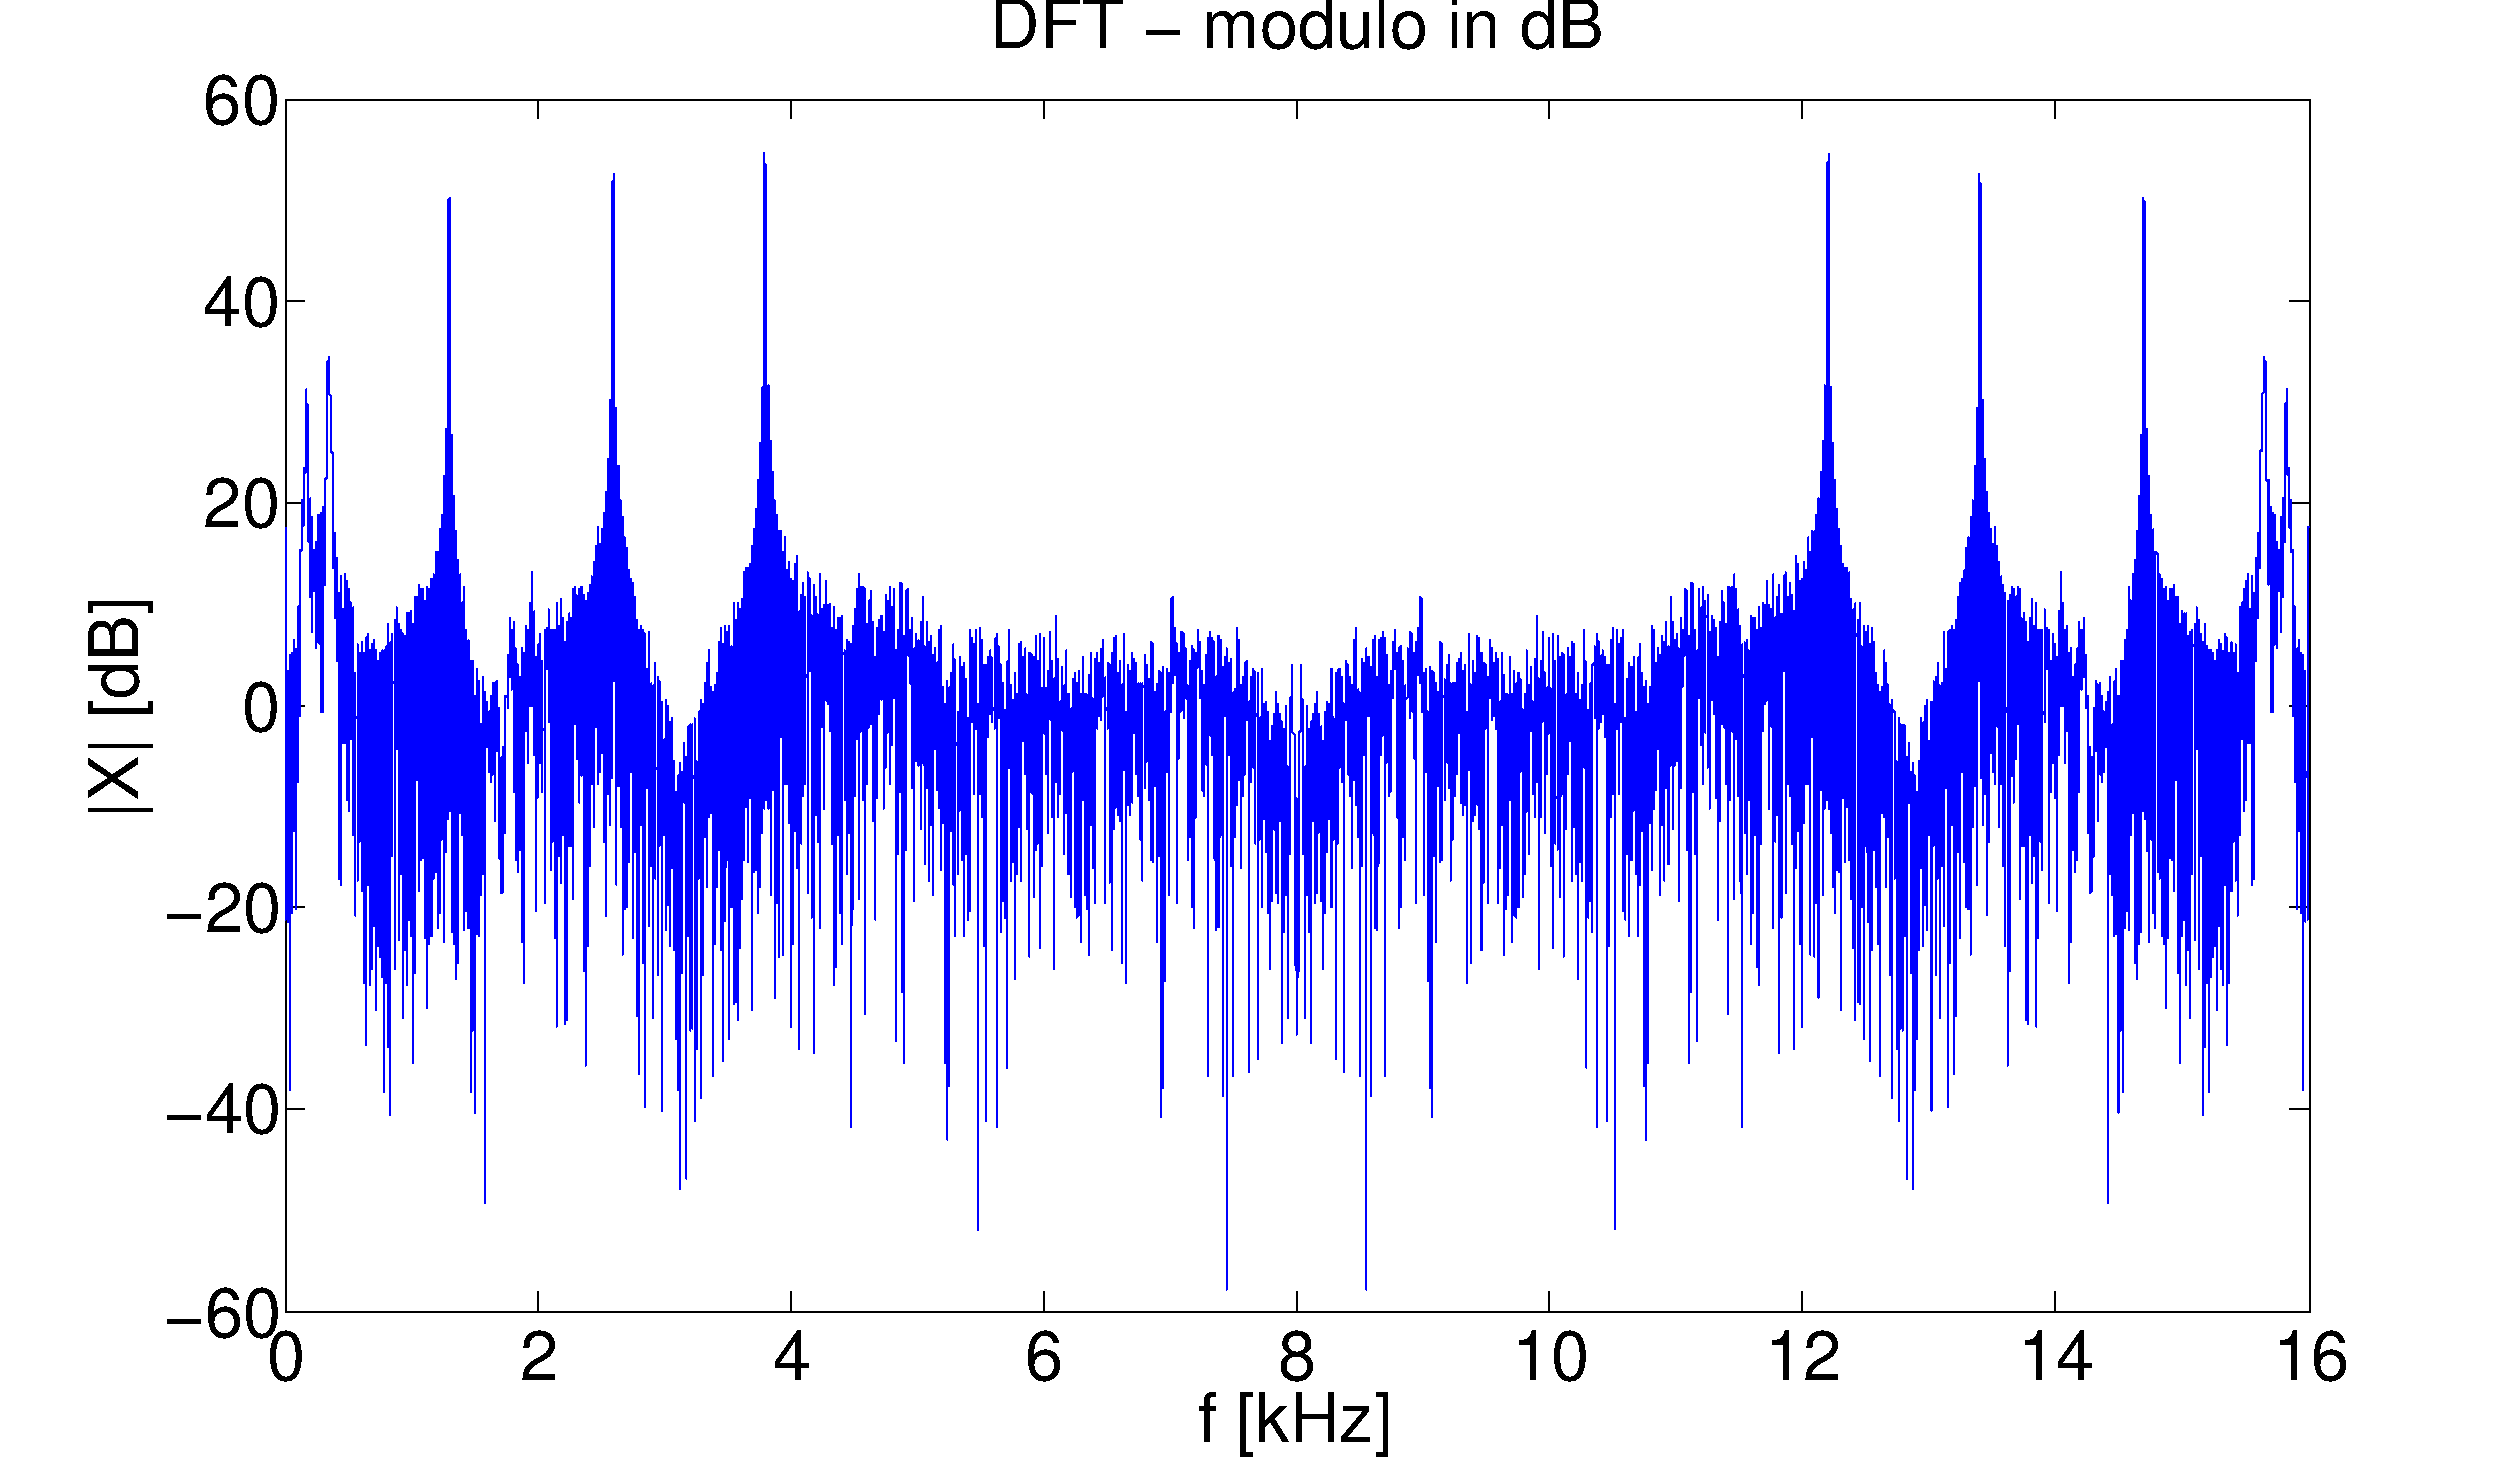
\includegraphics[width = 1\textwidth, keepaspectratio]{images/DFTdB.pdf}
  \caption{DFT di 250 ms di segnale con rumore a frequenza $f_1$ = 1300 Hz, $f_2$ = 2600 Hz, $f_3$ = 3800 Hz}
  \label{fig:unfilt}
\end{figure}

La prominenza della rappresentazione in frequenza di un seno sulla parte utile del segnale è ciò che consente di identificare le componenti sinusoidali in modo automatico. In particolar modo, data la DFT del segnale, si possono cercare i massimi per le frequenze da 0 a $F_s/2$. Le frequenze corrispondenti saranno quelle dei seni da rimuovere. Tuttavia, nel momento in cui si opera in real-time e non sull'intero segnale già registrato non si può sapere se nell'intervallo che si sta analizzando sia presente un rumore sinusoidale o meno. La strategia adottata pertanto deve tenere conto di questo fattore. Di seguito si propone lo pseudocodice~\ref{sinDet}. \\

\begin{algorithm}
  \caption{Procedura per rilevare rumore sinusoidale}\label{sinDet}
  \begin{algorithmic}[1]
    \Procedure{}{}
    \State dato $x(nT)$, segnale d'ingresso con
    \State $F_s$ frequenza di campionamento
    \State applica una finestra triangolare, ottenendo $y(nT)$
    \State definisce una soglia $R$
    \State calcola $X(e^{j\theta}) = DFT(x(nT))$
    \State calcola $Y(e^{j\theta}) = DFT(y(nT))$
    \While {$ max_{\theta \in [0, \pi]}(Y(e^{j\theta})) > R$}
    \State $f_j = \frac{F_s}{2\pi} \argmax_{\theta \in [0, \pi]}(Y(e^{j\theta}))$
    \State filtra la componente sinusoidale a frequenza $f_j$ in $X(e^{j\theta})$ e $Y(e^{j\theta})$
    \EndWhile
    \State $out(nT) = IDFT(X(e^{j\theta}))$
    \EndProcedure
  \end{algorithmic}
\end{algorithm}

In questo modo si riescono a identificare tutti i picchi più alti della soglia $R$, senza assunzioni preliminari sul numero di componenti sinusoidali presenti in un dato istante. L'approccio iterativo della procedura è ispirato all'articolo \cite{iterative}, in cui si propone un metodo per isolare componenti sinusoidali da un rumore bianco. In questa versione tuttavia lo scopo è eliminare le componenti sinusoidali rumorose dal parlato, che non ha una caratterizzazione statistica come il rumore bianco, pertanto non è stata ricavata una formulazione analitica per la soglia $R$. Questa è infatti costante e viene impostata applicando l'algoritmo su diversi campioni audio (solo parlato, parlato e componenti sinusoidali) e identificando quale valore consente di discriminare le sinusoidi del rumore dalle fondamentali della voce nella maggiorparte dei casi. Queste ultime sono infatti sinusoidi, se osservate in un intervallo sufficientemente stretto, ma di ampiezza inferiore rispetto a quella del rumore da eliminare, che tende a saturare e quindi raggiungere il massimo valore rappresentabile. \\
L'utilizzo di una finestra triangolare consente di abbassare i picchi laterali dei seni, in questo modo lo \textit{spectral leackage} diminuisce e aumenta la differenza in ampiezza tra i picchi che rappresentano un seno e quelli che rappresentano le fondamentali della voce. Si possono quindi usare soglie $R$ più basse, identificando il rumore sinusoidale anche quando si sta sviluppando e non è in saturazione. Inoltre l'utilizzo della finestra triangolare consente di distinguere eventuali seni con frequenze vicine. \\


\section{Filtri Notch IIR del second'ordine}
Per rimuovere le componenti sinusoidali dal segnale utile sono stati utilizzati dei filtri notch IIR del second'ordine.
Ciascun filtro ha risposta in frequenza
\begin{equation}
  H_j(e^{j\theta}) = b_0 \frac{1 - 2\cos\theta_0 e^{-j\theta} + e^{-j2\theta}}{1 - 2 r \cos\theta_0 e^{-j\theta} + r^2 e^{-j2\theta}}
\end{equation}
dove $\theta_0 = 2pif_j/F_s$, $r = (1 - \Delta\theta_{3dB} / 2)$, con $f_j$ frequenza da filtrare e $F_s$ frequenza di campionamento, $b_0 = 1$ \\
Nel campione da analizzare le frequenze $f_j$ a cui si sviluppano le componenti sinusoidali sono riportate in Figura~\ref{fig:unfilt}. Modulo e fase dei singoli filtri applicati su ciascuna componente si possono vedere nelle Figure~\ref{fig:1300},~\ref{fig:2600},~\ref{fig:3800}, mentre modulo e fase della cascata dei 3 filtri sono nelle Figure~\ref{fig:modtot} e~\ref{fig:phtot}. Per ciascuno $\Delta\theta_{3dB} = 200 $ Hz, $ F_s = 16 $ KHz. \\
La fase di questi filtri non è lineare, ma non è un requisito necessario per il filtraggio di segnali audio. \\


\begin{figure}[h!]
  \centering
  \subfigure[Modulo]{
    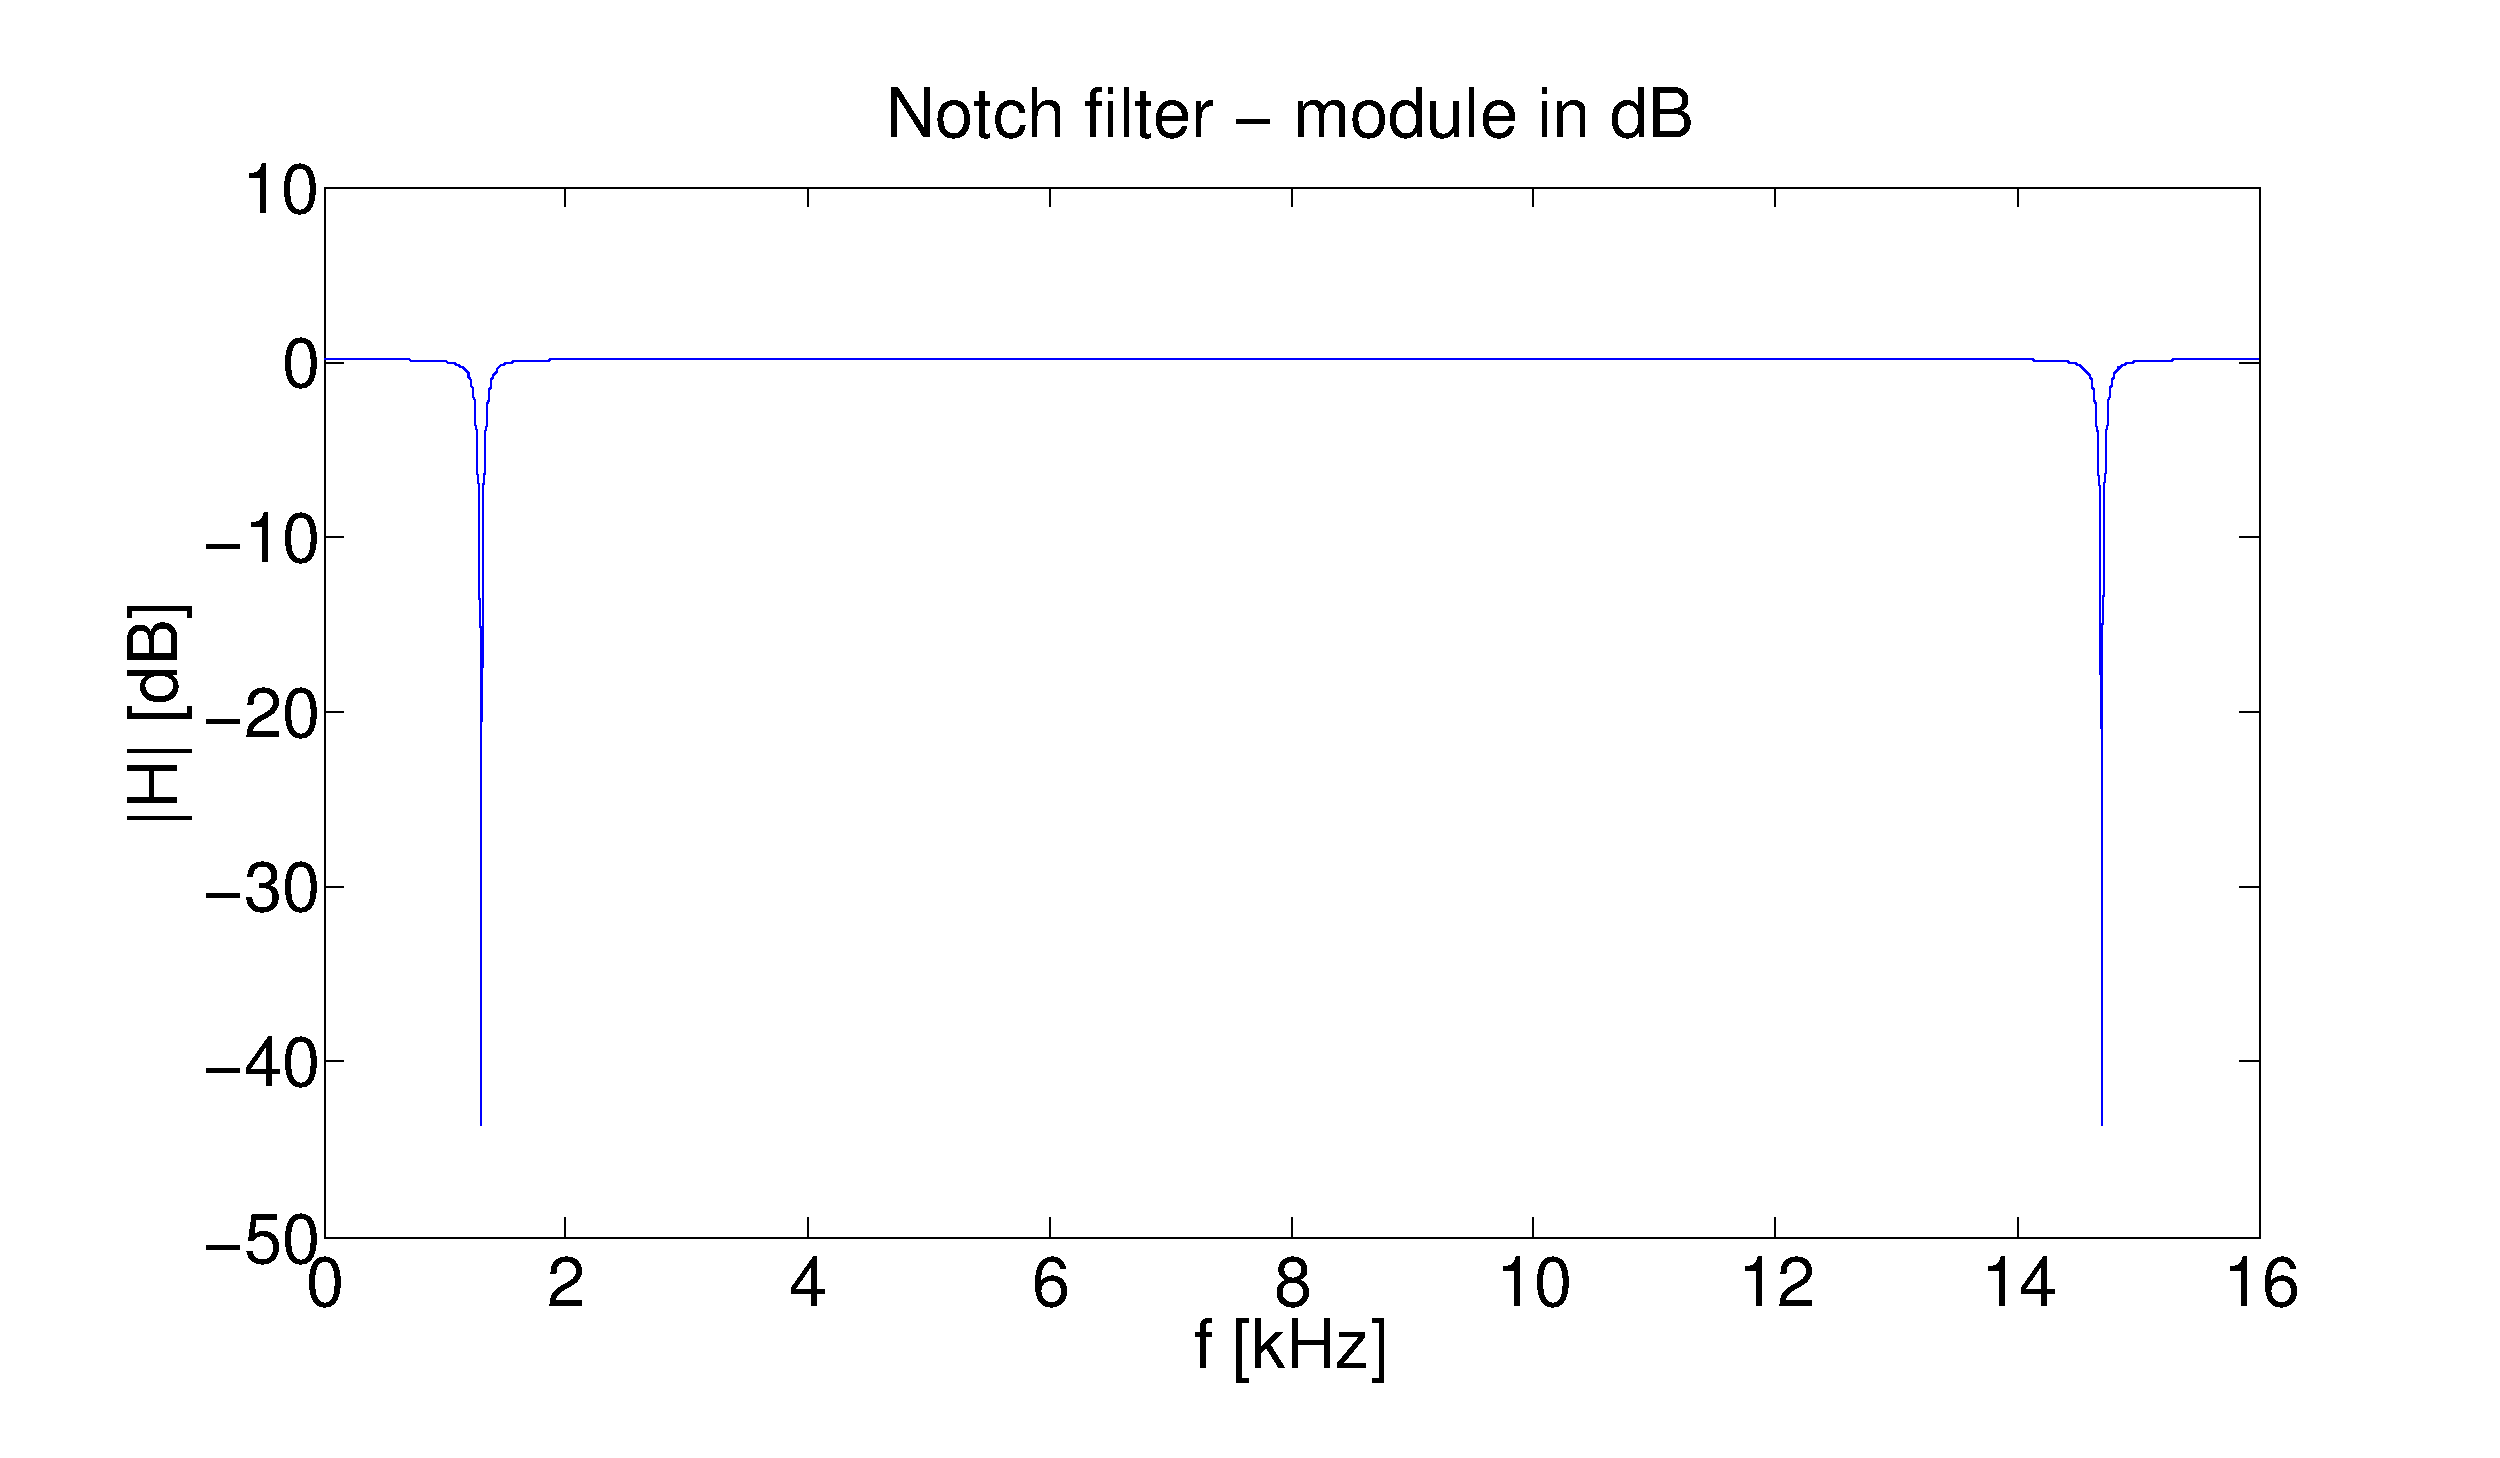
\includegraphics[width = 0.45\textwidth, keepaspectratio]{images/notch1300mod.pdf} }
  \subfigure[Fase]{
    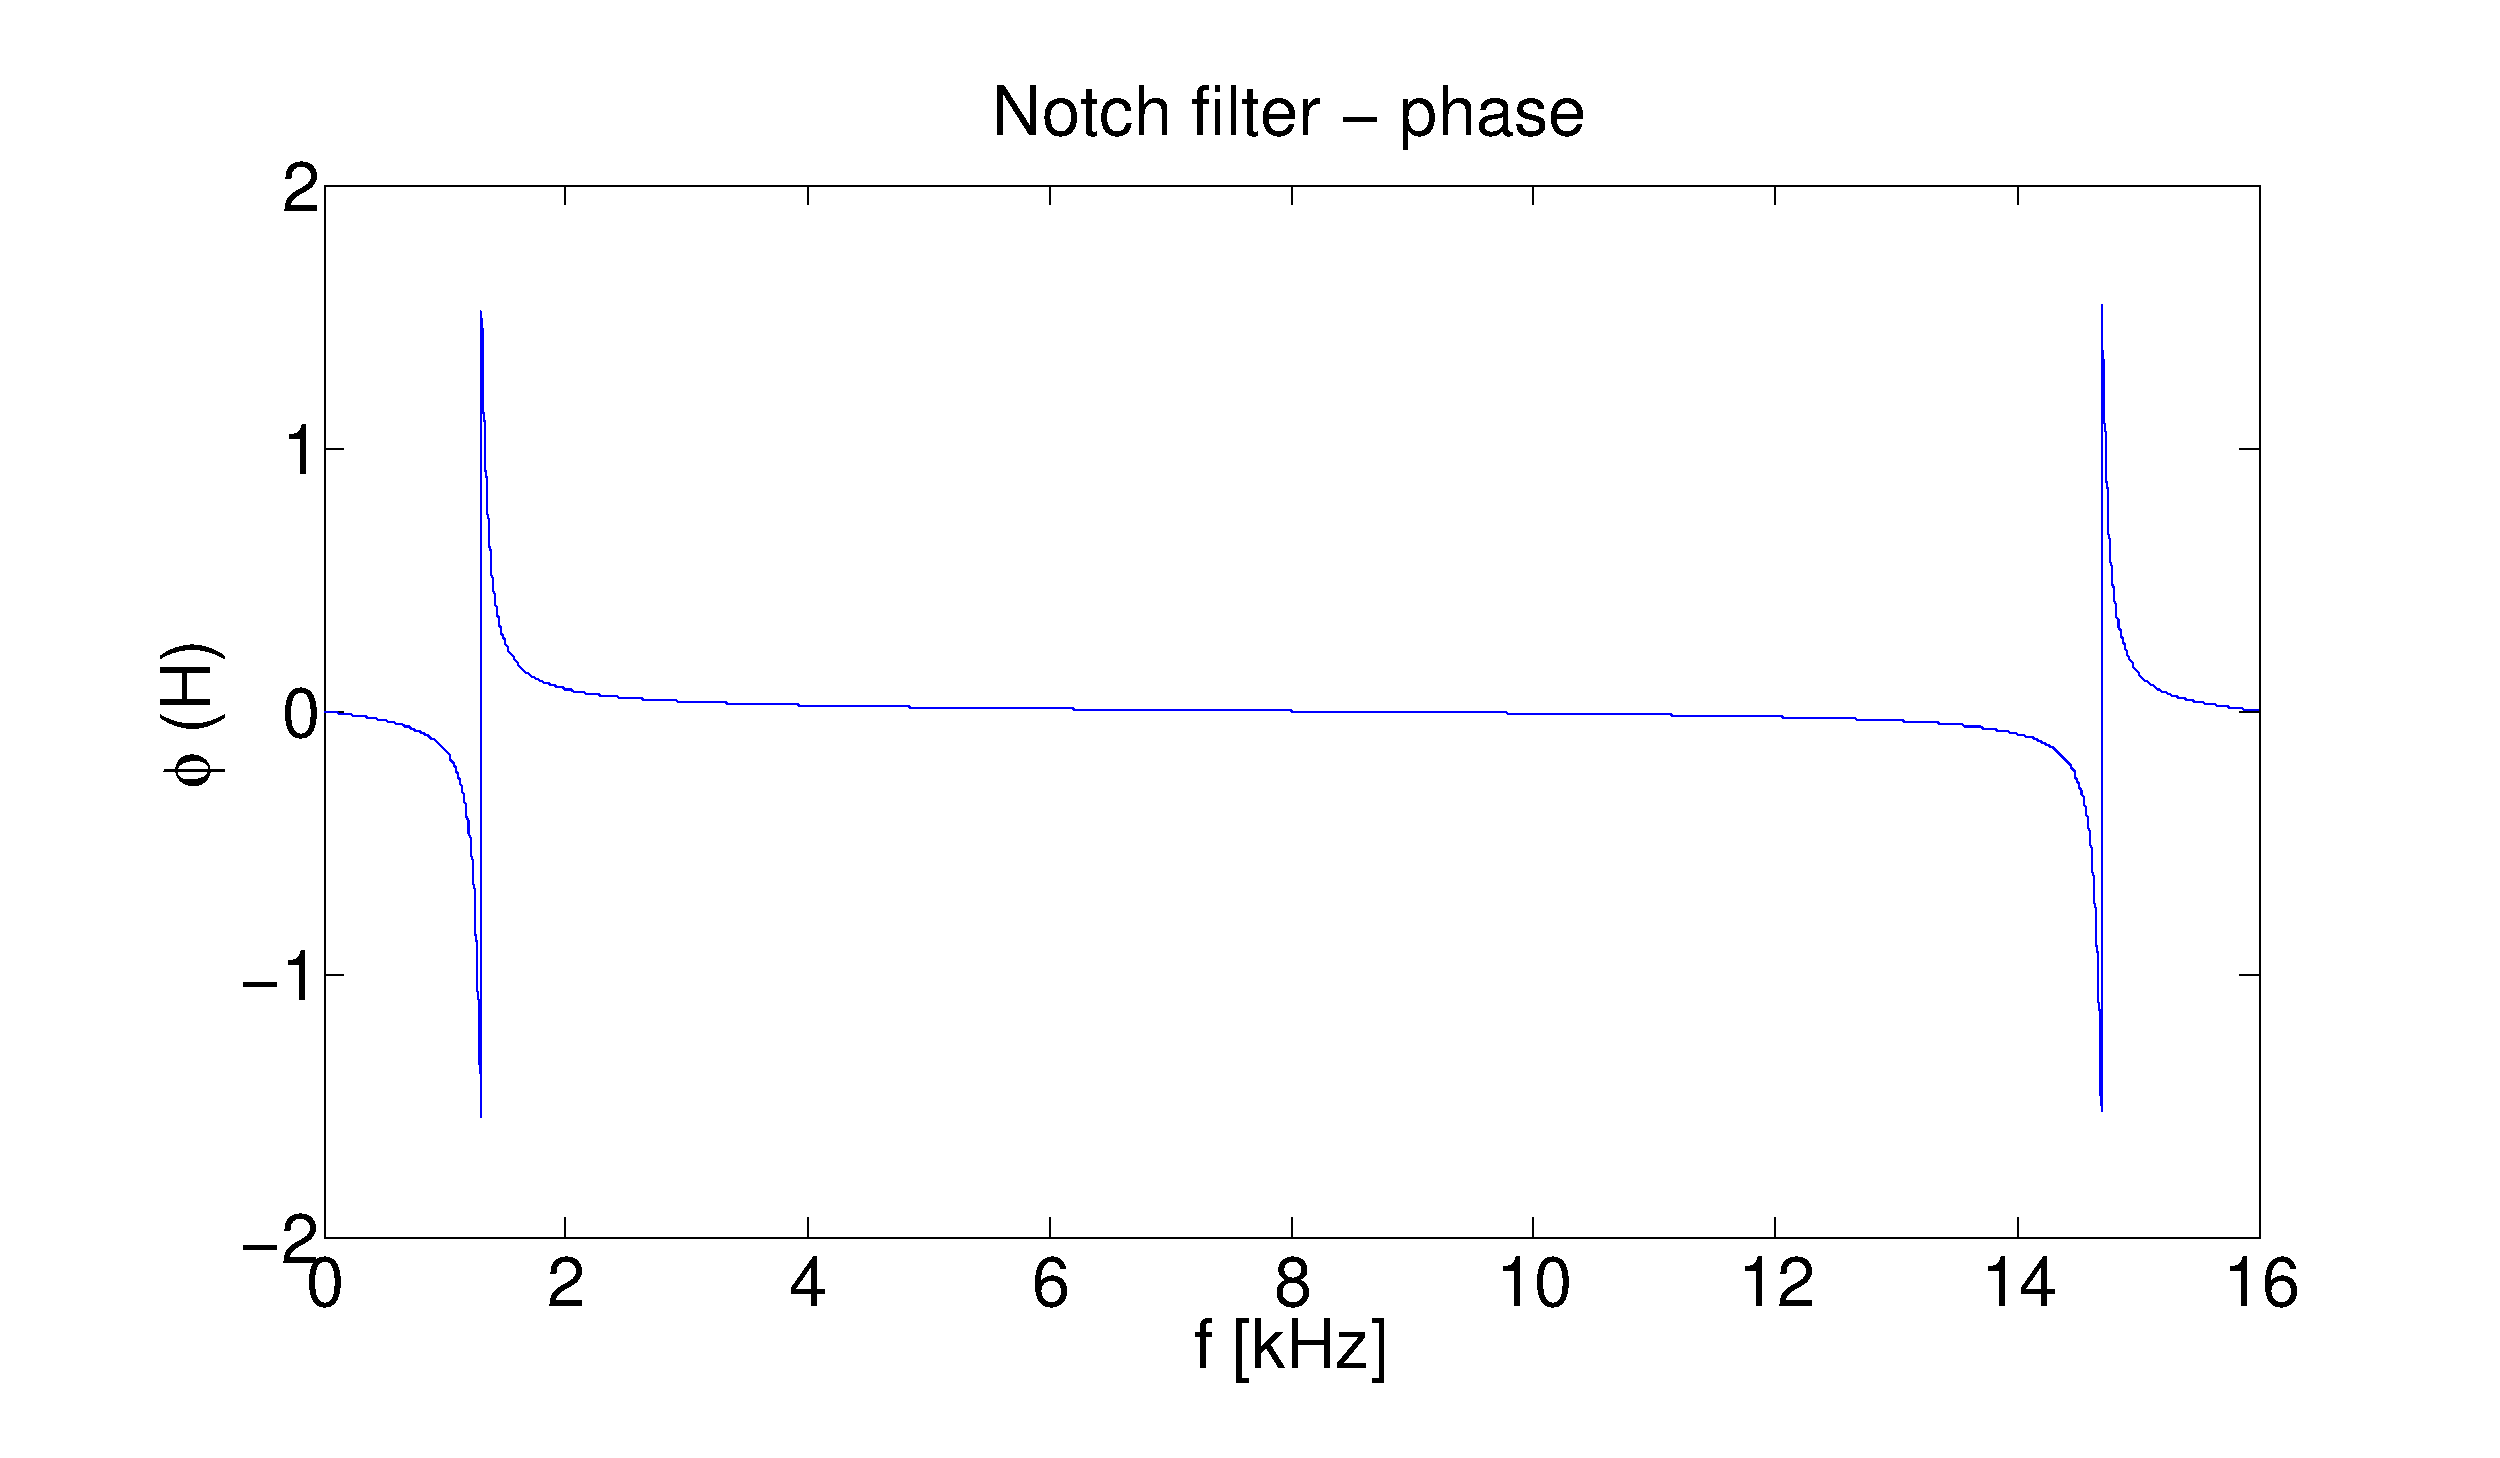
\includegraphics[width = 0.45\textwidth, keepaspectratio]{images/notch1300ph.pdf}}
  \caption{Filtro notch per f = 1300 Hz}
  \label{fig:1300}
\end{figure}

\begin{figure}[h!]
  \centering
  \subfigure[Modulo]{
  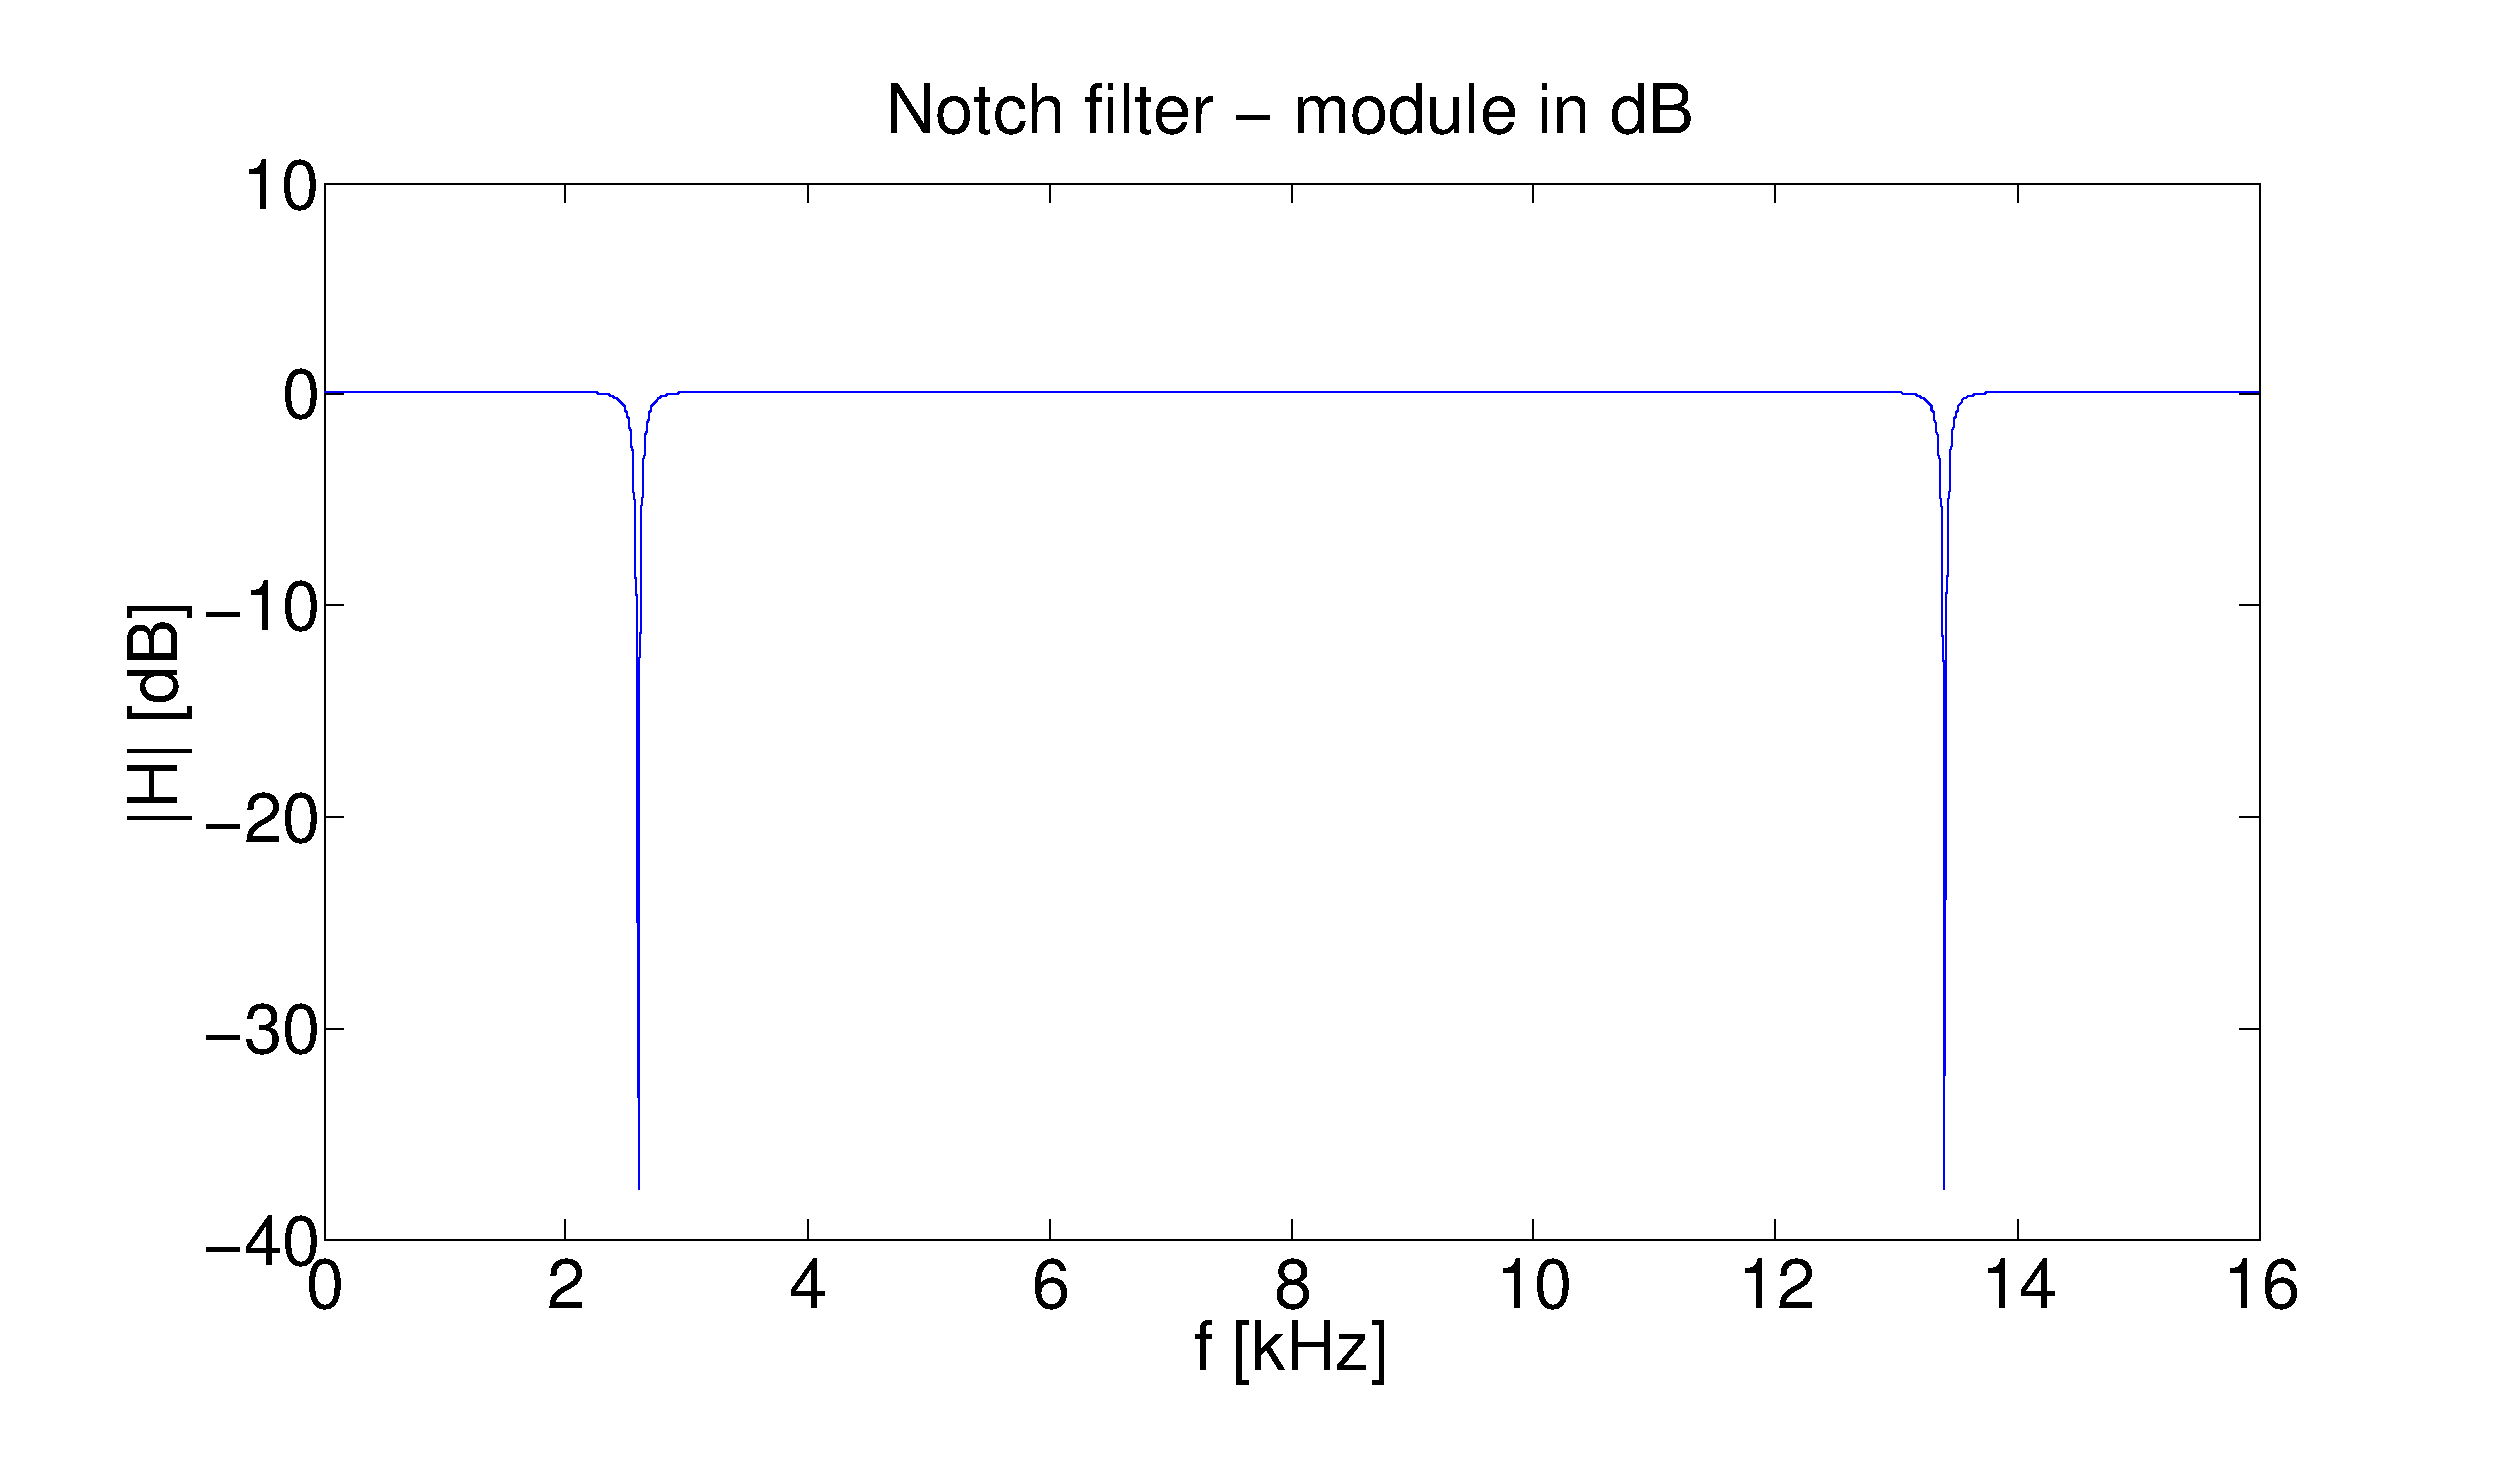
\includegraphics[width = 0.45\textwidth, keepaspectratio]{images/notch2600mod.pdf} }
  \subfigure[Fase]{
  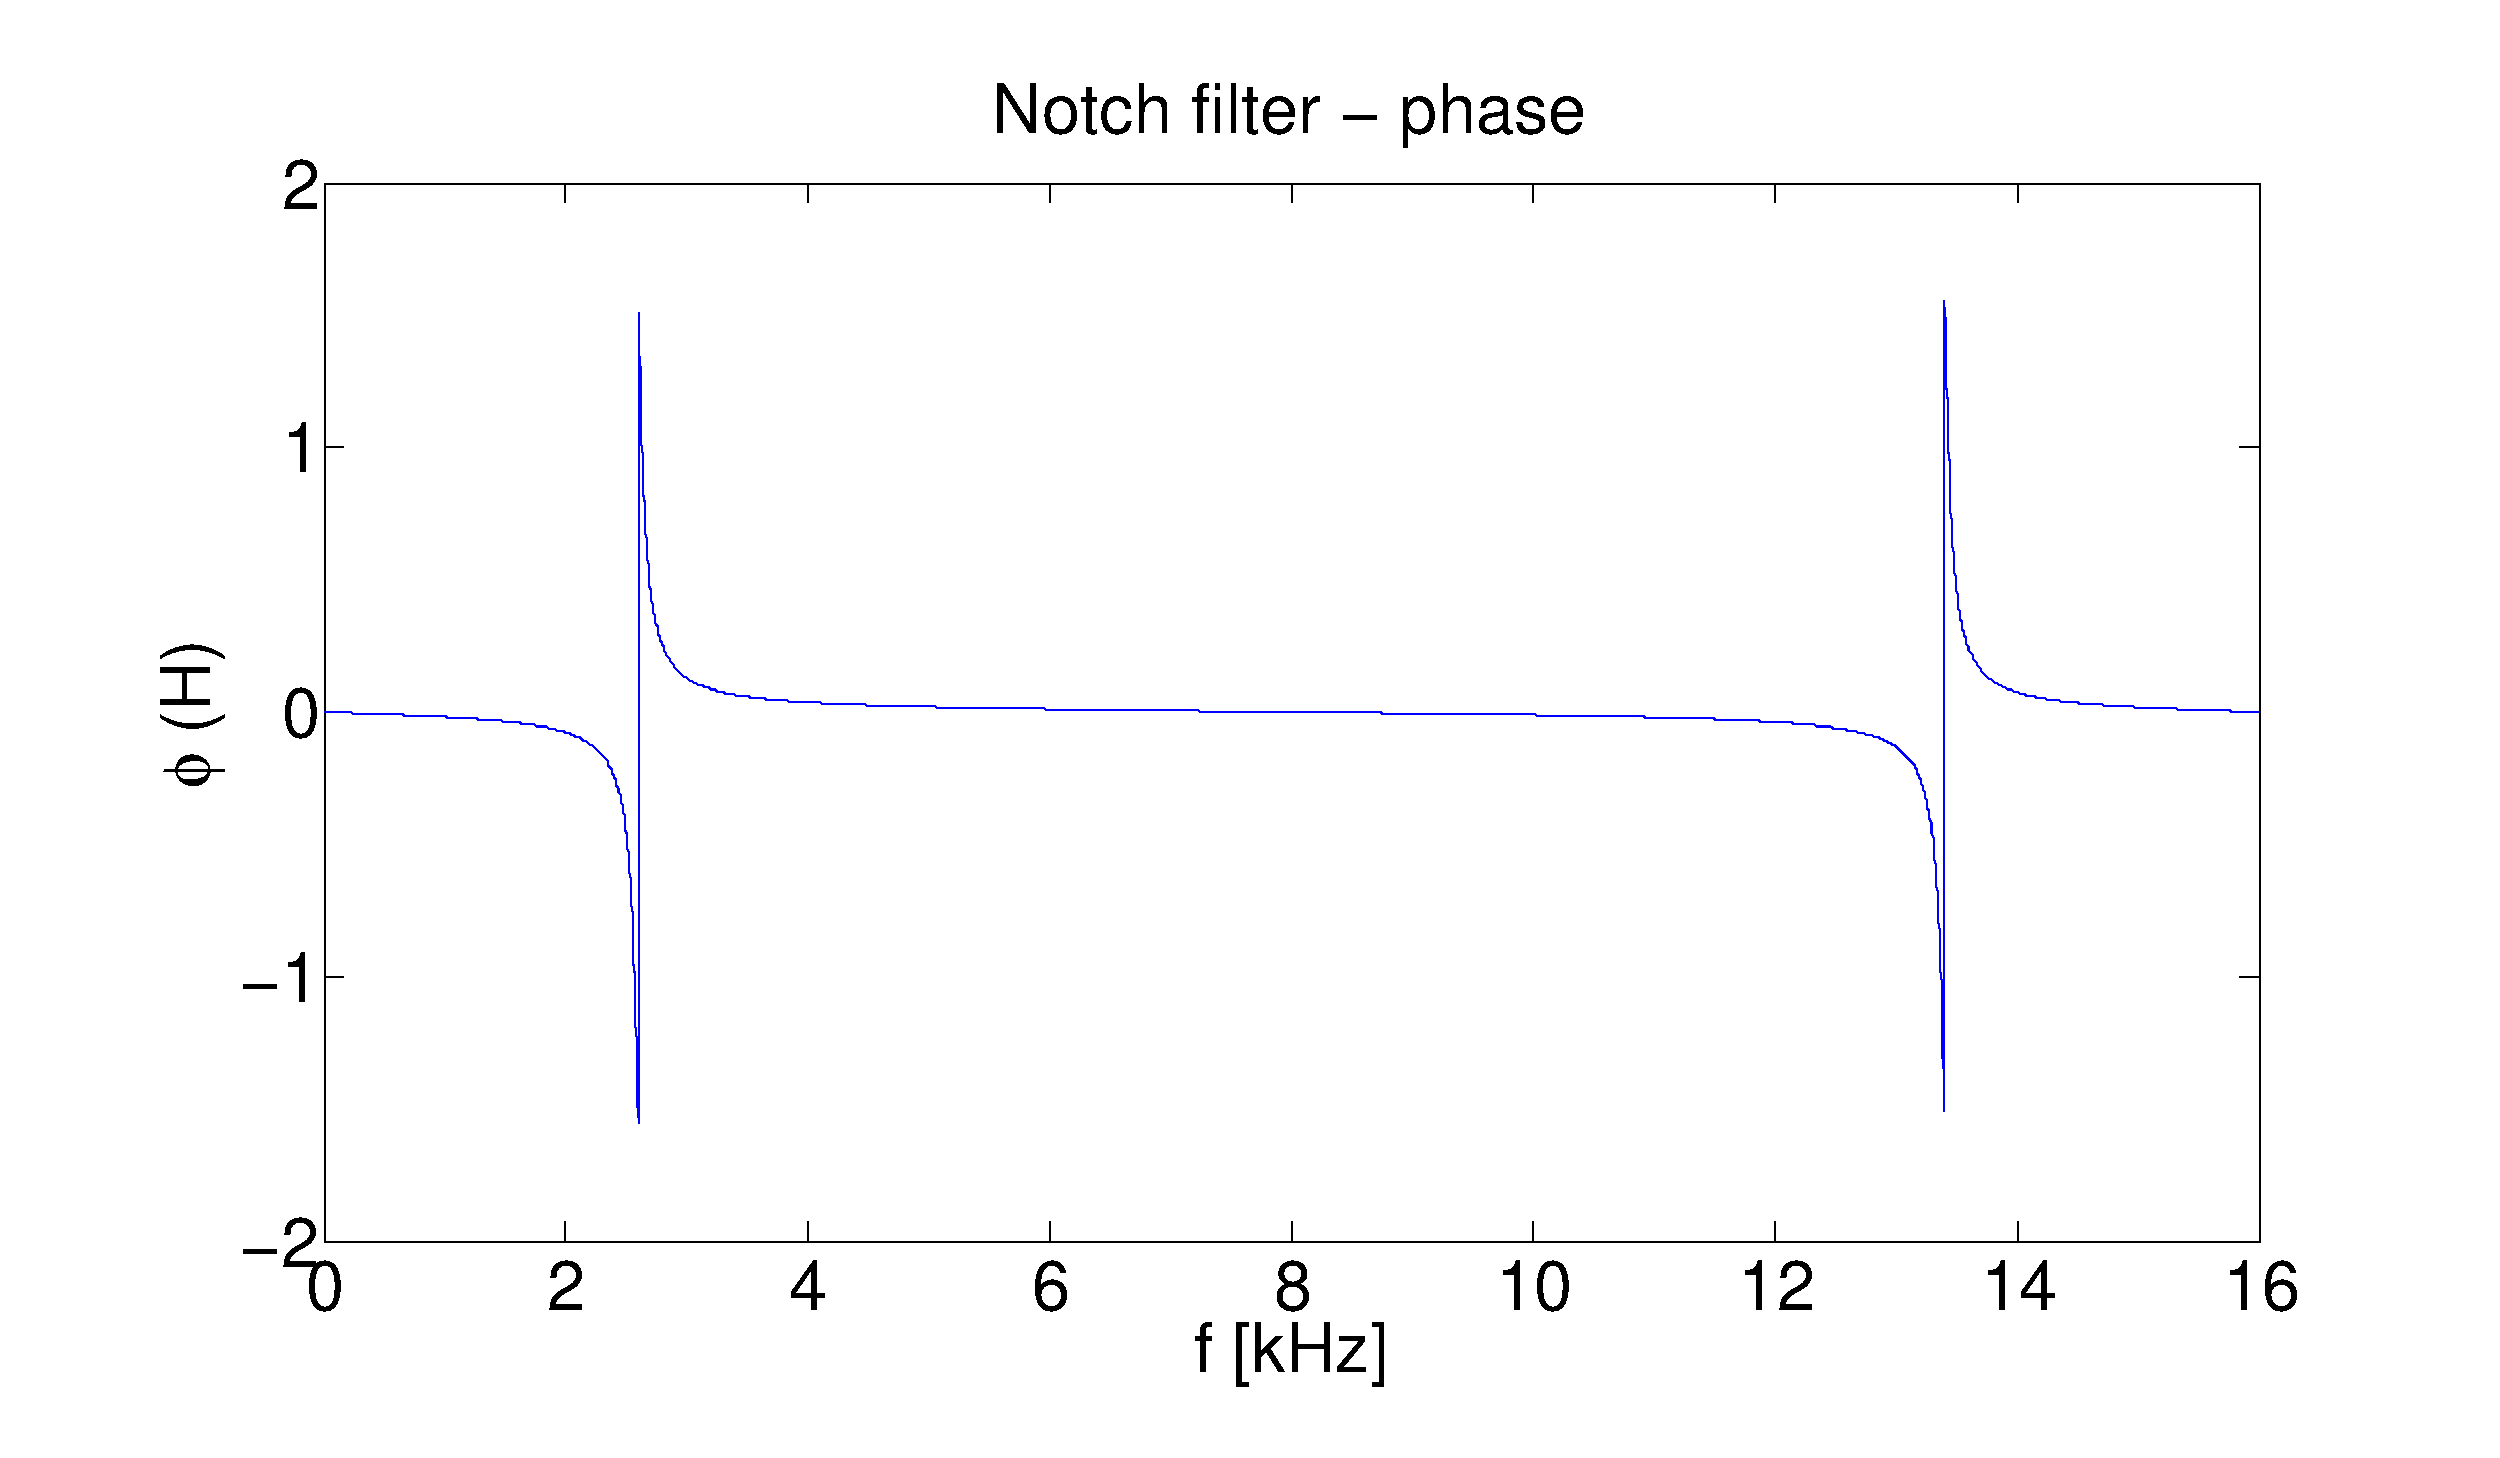
\includegraphics[width = 0.45\textwidth, keepaspectratio]{images/notch2600ph.pdf}}
  \caption{Filtro notch per f = 2600 Hz}
  \label{fig:2600}
\end{figure}

\begin{figure}[h!]
  \centering
  \subfigure[Modulo]{
  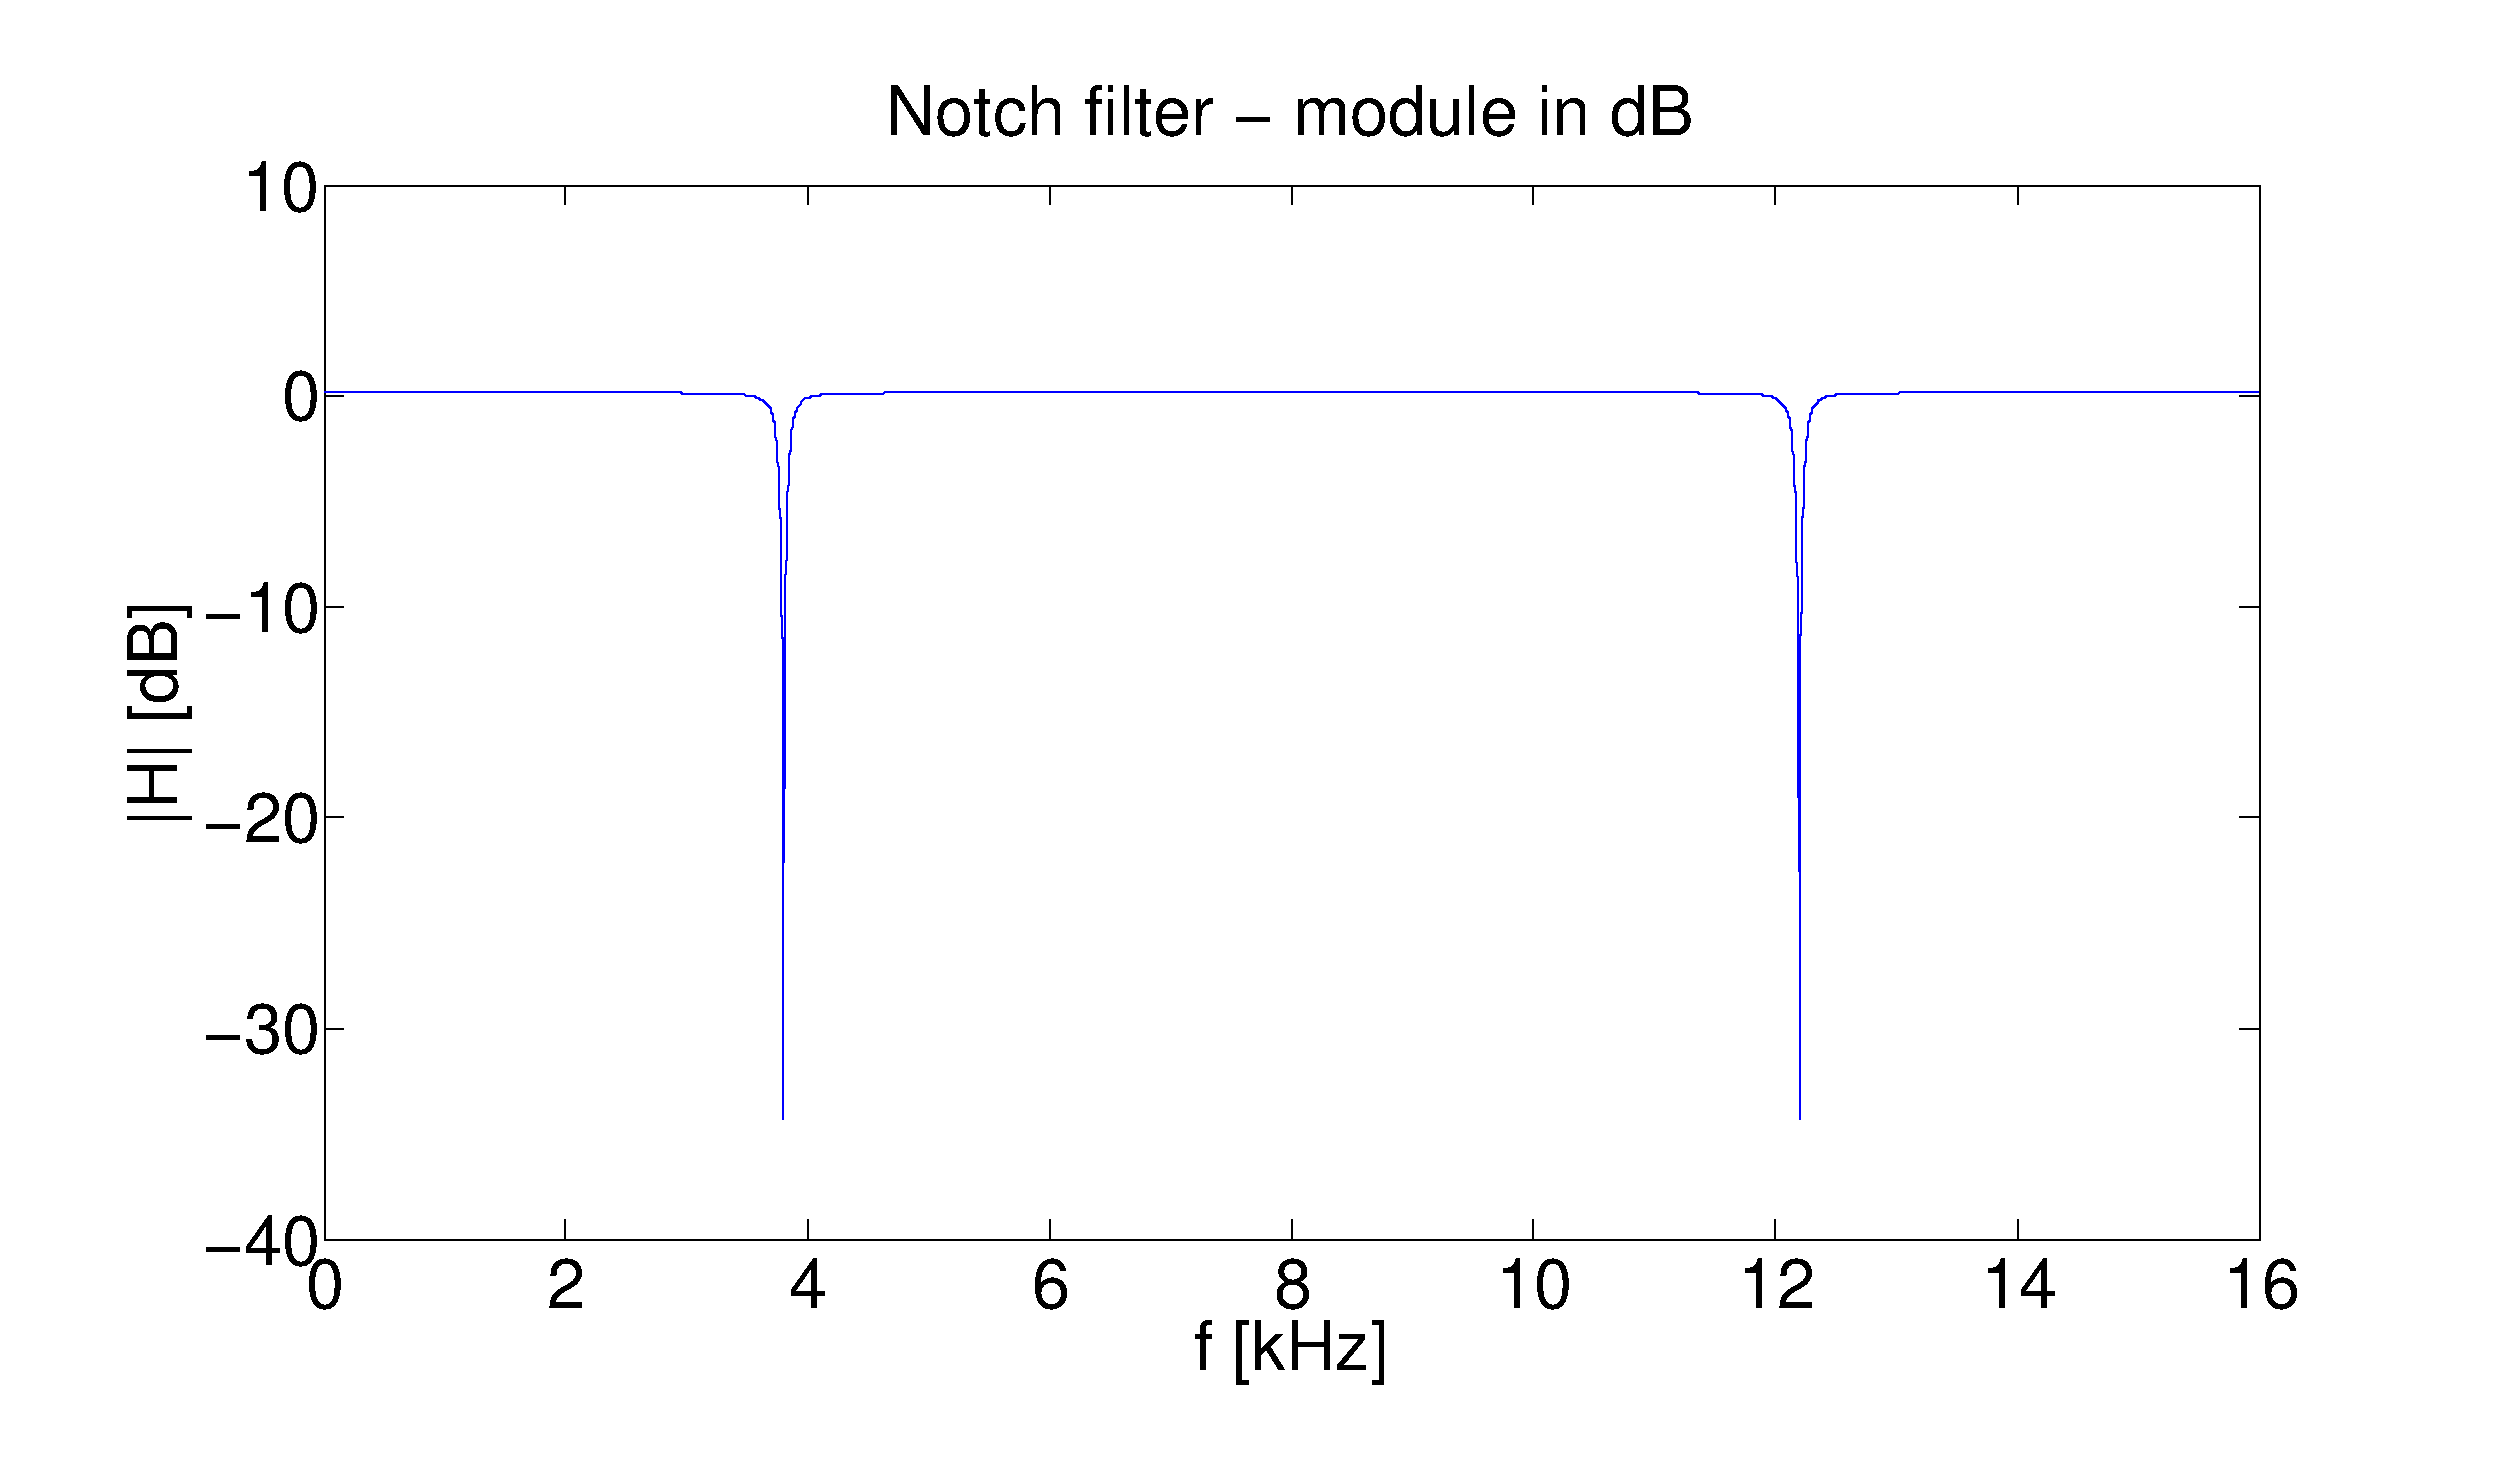
\includegraphics[width = 0.45\textwidth, keepaspectratio]{images/notch3800mod.pdf} }
  \subfigure[Fase]{
  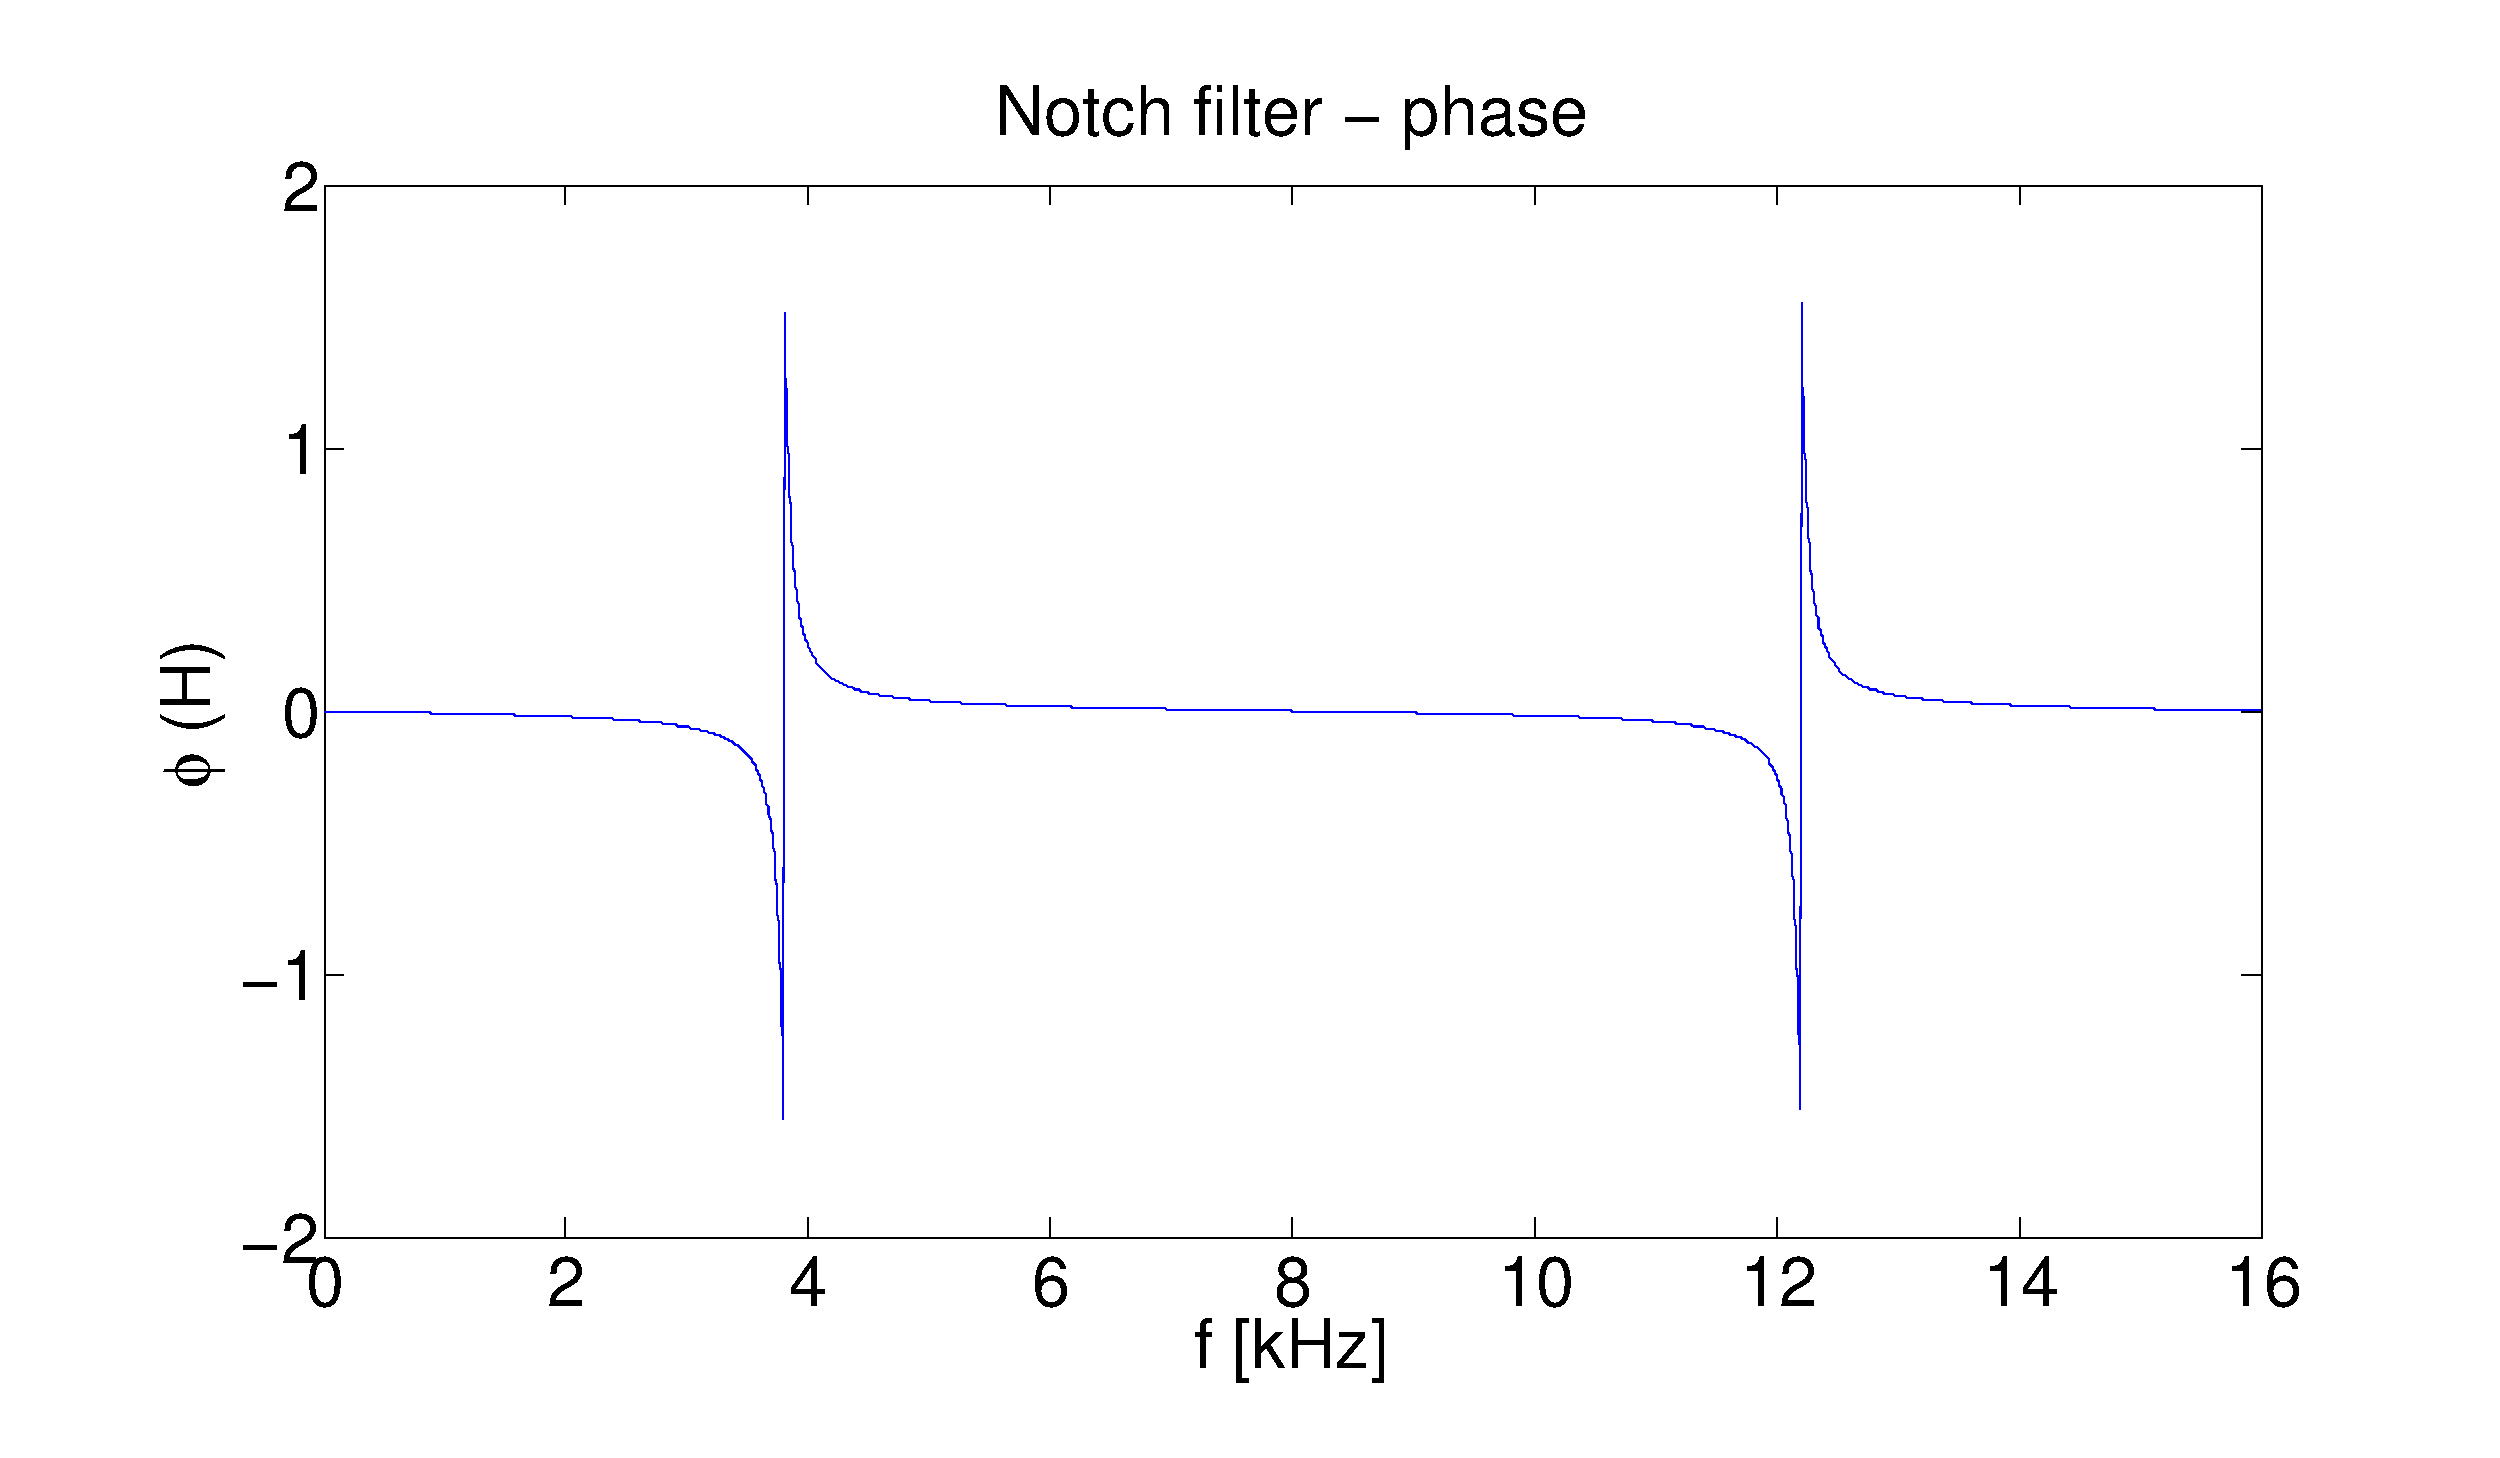
\includegraphics[width = 0.45\textwidth, keepaspectratio]{images/notch3800ph.pdf}}
  \caption{Filtro notch per f = 3800 Hz}
  \label{fig:3800}
\end{figure}

\clearpage

\begin{figure}[h!]
  \centering
  \includegraphics[width = 1\textwidth, keepaspectratio]{images/NotchTotMod.pdf}
  \caption{Modulo della cascata dei 3 filtri notch}
  \label{fig:modtot}
\end{figure}

\begin{figure}[h!]
  \centering
  \includegraphics[width = 1\textwidth, keepaspectratio]{images/NotchTotPh.pdf}
  \caption{Fase della cascata dei 3 filtri notch}
  \label{fig:phtot}
\end{figure}

\clearpage

\section{Implementazione in MATLAB$^{\circledR}$}
Il campione audio da analizzare presenta rumore sinusoidale con una componente da 3 s a 5 s a frequenza 1300 Hz, la precedente e un seno di frequenza 2600 Hz da 5 s a 6 s e infine si aggiunge una sinusoide a frequenza 3800 Hz fino alla fine del segnale (10 s). In Figura~\ref{fig:nsins} si può trovare l'andamento del numero di seni nel tempo.\\

\begin{figure}[h!]
  \centering
  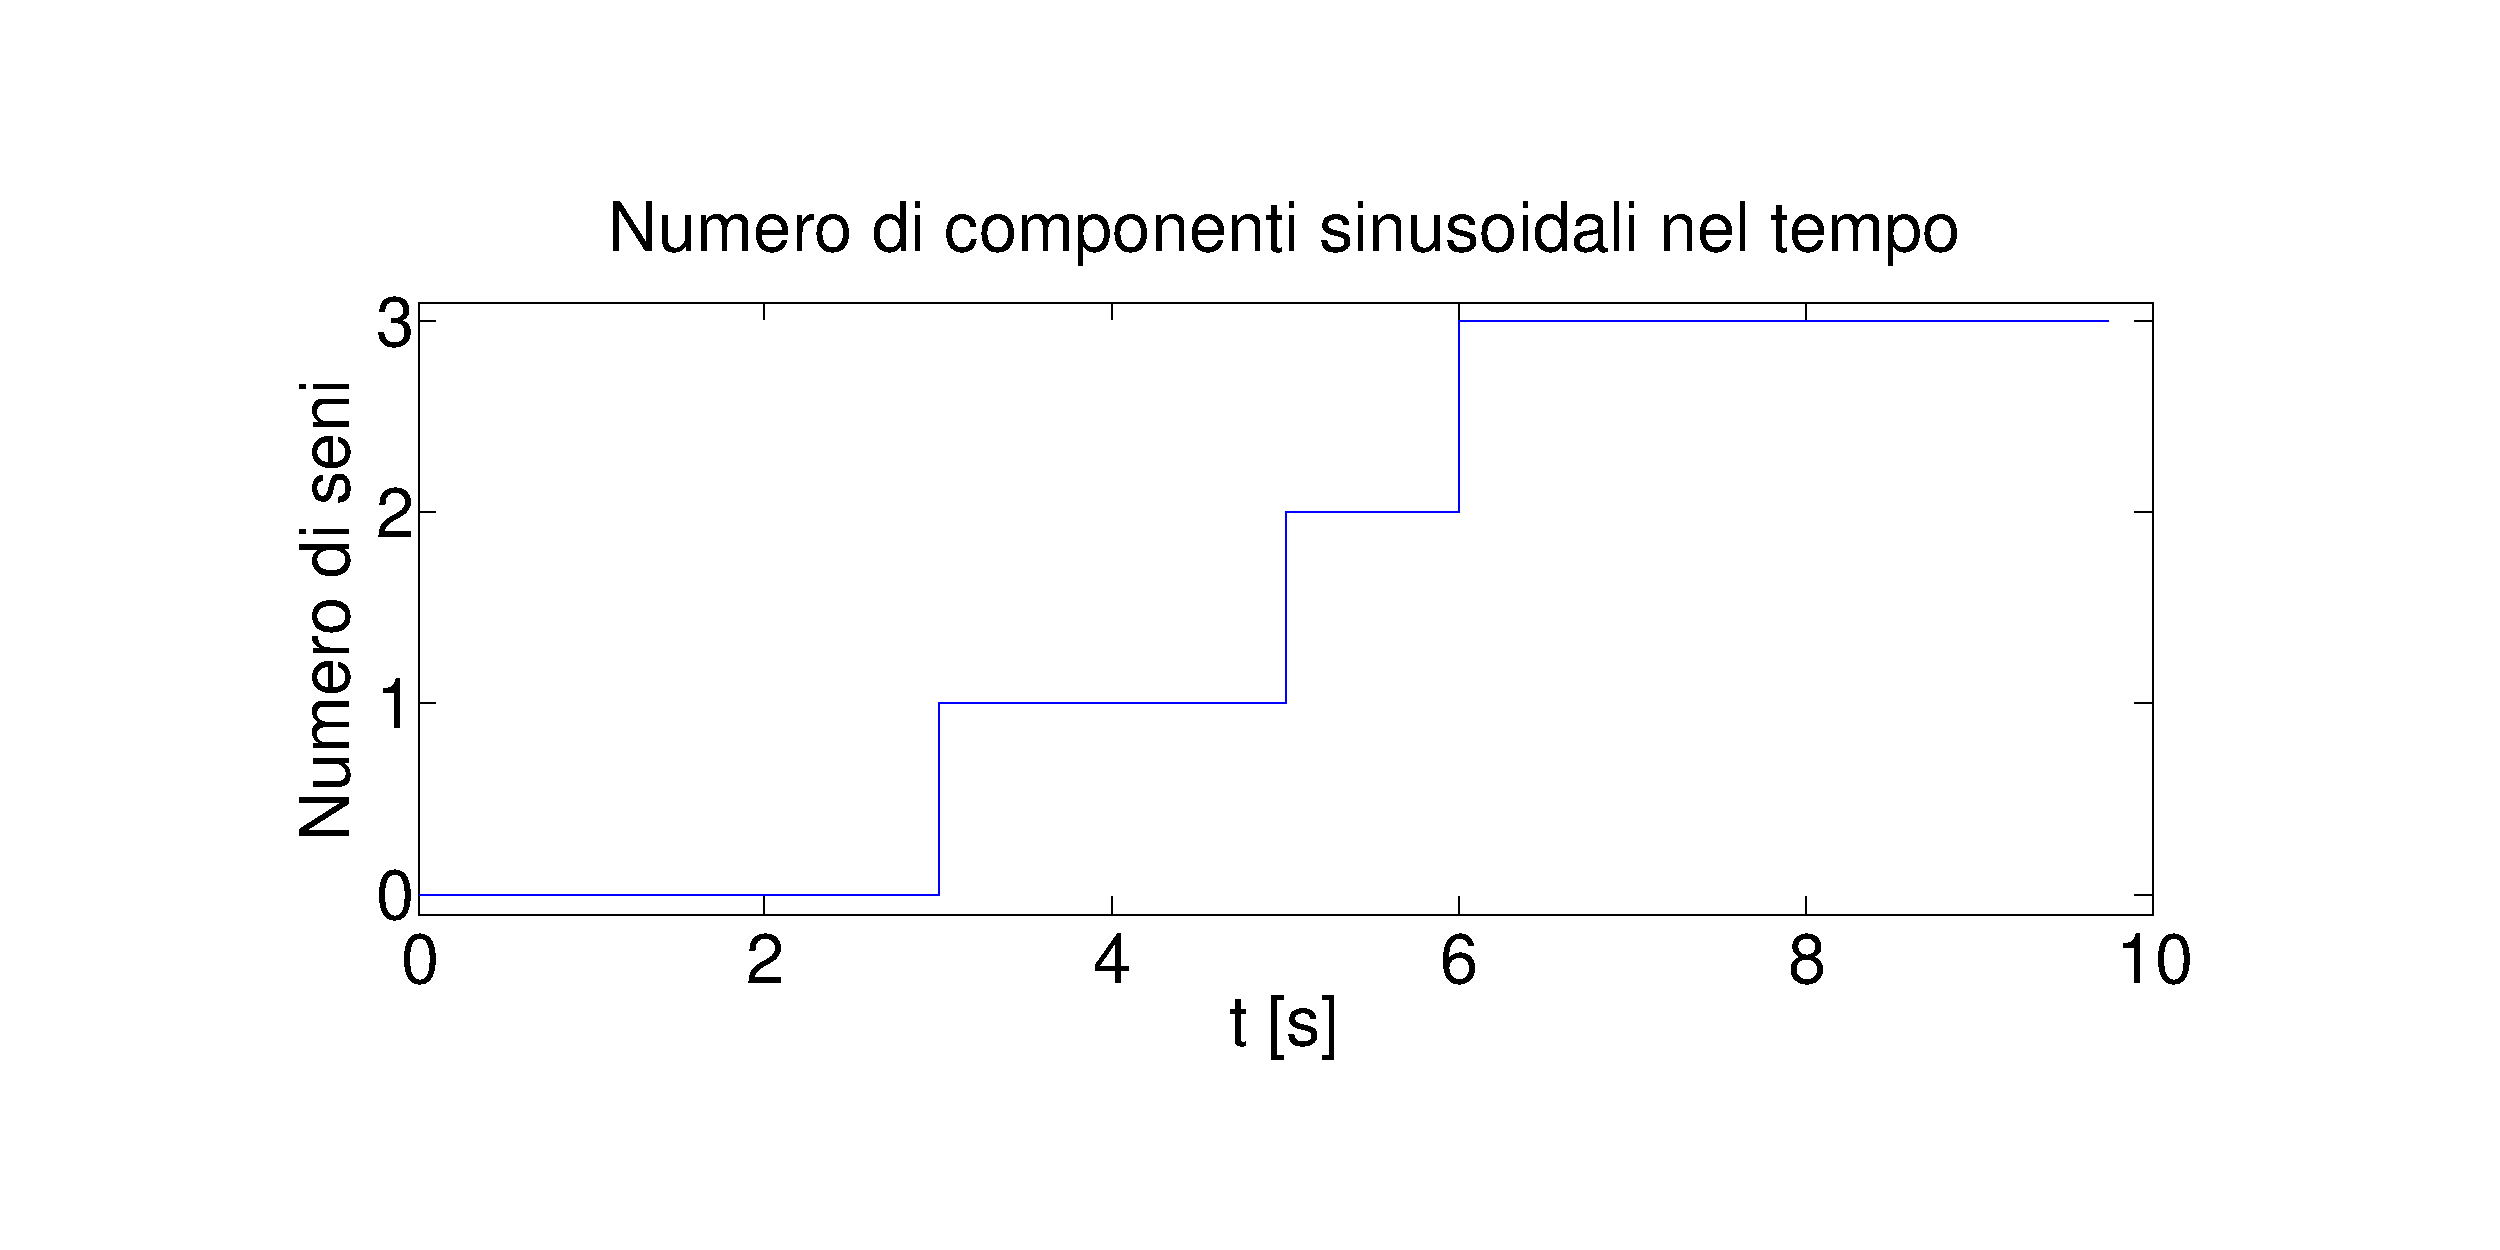
\includegraphics[width=\textwidth, trim = 0 90 0 90, clip = true,  keepaspectratio]{images/seniTempo.pdf}
  \caption{Numero di componenti sinusoidali nel tempo}
  \label{fig:nsins}
\end{figure}

L'implementazione dell'algoritmo~\ref{sinDet} è stata realizzata in real-time grazie all'utilizzo del package \texttt{dsp} di MATLAB$^{\circledR}$. L'approccio seguito è quello di filtrare $n$ samples del segnale prima e riprodurre gli stessi in seguito, mentre si filtrano gli $n$ successivi. Quindi in realtà è presente una latenza che è pari a $n/F_s$, con $F_s$ frequenza di campionamento. La DFT è calcolata usando la funzione \texttt{fft}.\\
Di seguito il codice utilizzato, con \texttt{systobjdemo} che ha il compito di acquisire il segnale, filtrarlo e riprodurlo $n$ samples per volta. Il rilevamento dei rumori sinusoidali e l'effettivo filtraggio è svolto dal System Object \texttt{deleteSins}.\\
Durante lo sviluppo del codice sono state effettuate alcune osservazioni. Innanzitutto c'è un trade-off tra la qualità del segnale filtrato, le risorse computazionali richieste e la latenza ammessa. Con la procedura~\ref{sinDet} si riescono ad isolare e filtrare le componenti sinusoidali, senza filtrare anche fondamentali della voce, con una latenza minima di 125 ms, ovvero sia è necessario utilizzare almeno 2000 campioni del segnale. Al di sotto di questa soglia il sistema funziona ma riconosce come seno anche qualche vocale, in particolar modo le ``i''. \\
Inoltre per identificare con precisione la frequenza delle sinusoidi è necessario introdurre uno \textit{zero padding} nella FFT, ovvero sia aumentare la risoluzione frequenziale a cui questa è calcolata. Identificare correttamente la frequenza del seno è fondamentale per poter applicare correttamente un filtro a banda stretta, che quindi non penalizzi il parlato, ma che consenta di rimuovere completamente il rumore. Errori nell'ordine di qualche Hertz lasciano un rumore di fondo distinguibile.\\
\newpage
\lstinputlisting[inputencoding=utf8/latin1]{code/systobjdemo.m}
\newpage


\lstinputlisting[inputencoding=utf8/latin1]{code/deleteSins.m}

\section{Risultati}
Sono state effettuate numerose prove per tarare al meglio i parametri del System Object \texttt{deleteSins}. Alla fine si è raggiunto un compromesso tra risorse computazionali allocate, latenza e qualità del segnale filtrato che consente di rimuovere il rumore sinusoidale pur operando con una latenza ridotta. A titolo esemplificativo, il risultato del filtraggio sul campione di Figura~\ref{fig:unfilt} è presente in Figura~\ref{fig:filt}. Come si può osservare le componenti sinusoidali sono state ridotte di circa 40 dB. Resta un rumore di fondo, dovuto al fatto che si è scelta una larghezza di banda ai 3 dB $\Delta\theta_{3dB} = 200$ Hz, per non penalizzare eccessivamente il segnale utile, e che si opera in real-time, quindi si ha a disposizione un numero di campioni limitato per effettuare l'analisi in frequenza. \\
Si rimanda al file .wav allegato per i risultati del filtraggio sul segnale completo.

\begin{figure}[h]
  \centering
  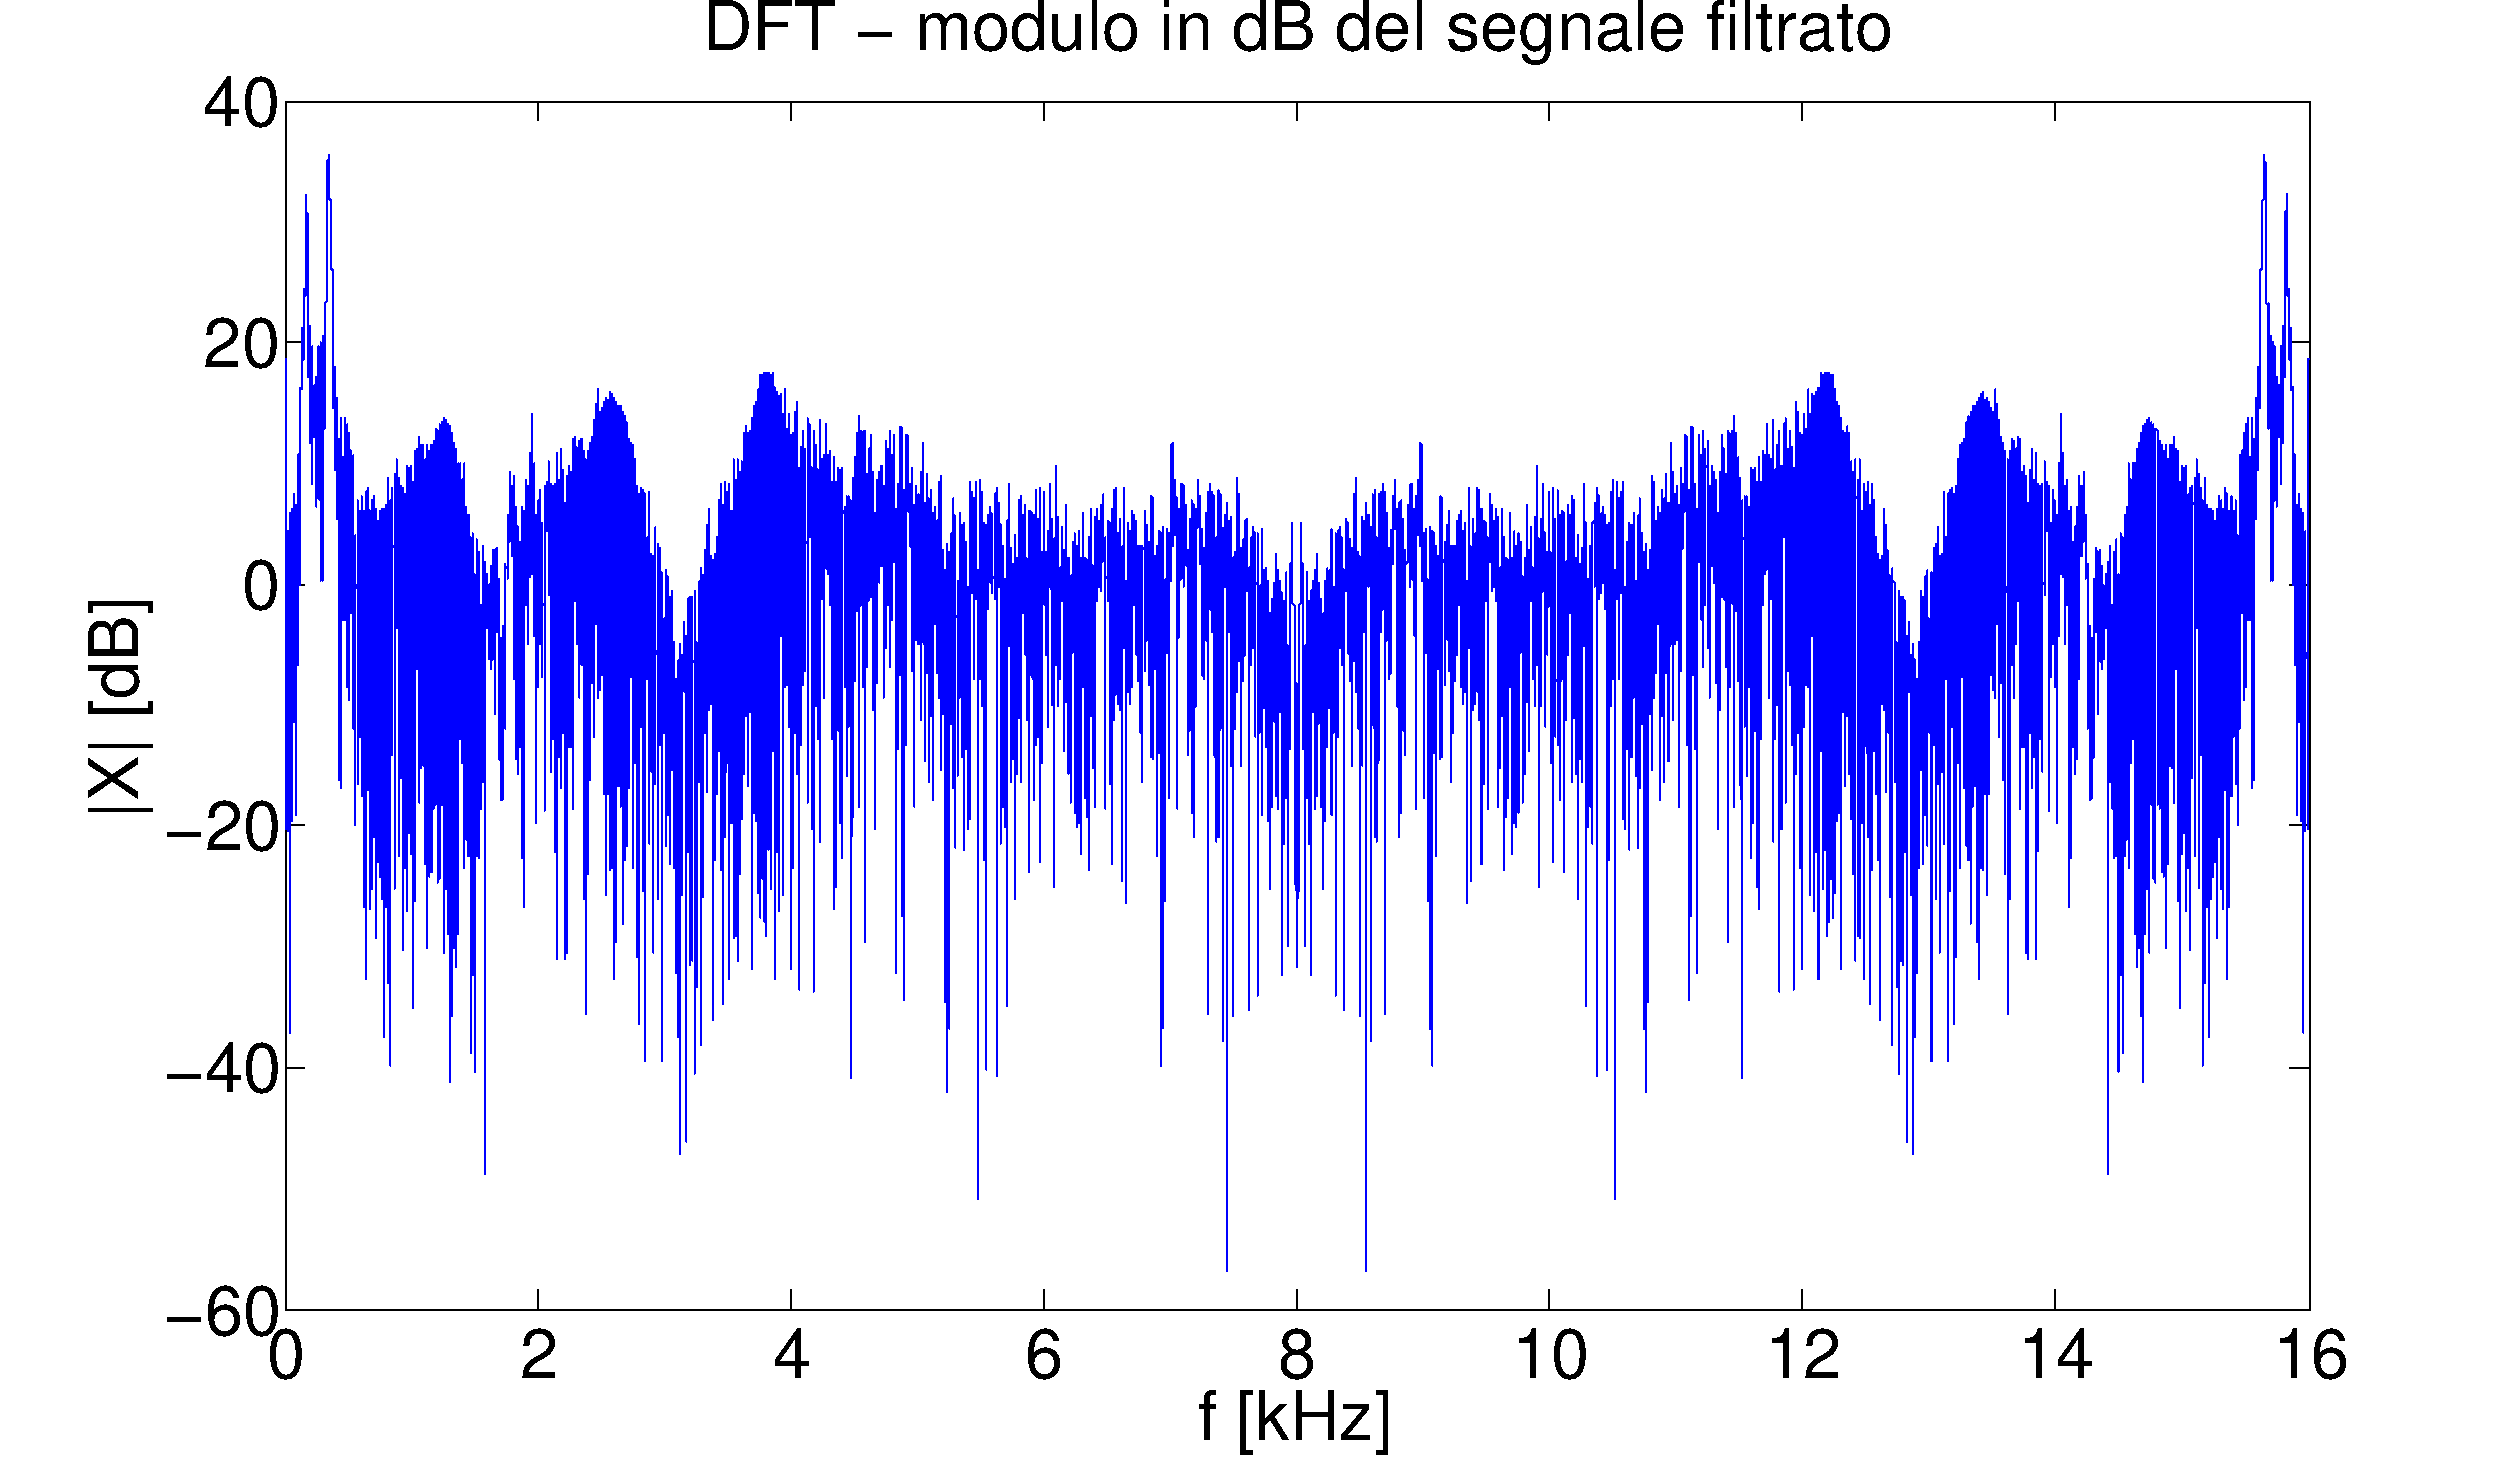
\includegraphics[width = 1\textwidth, keepaspectratio]{images/DFTdBFiltered.pdf}
  \caption{DFT di 250 ms di segnale filtrato}
  \label{fig:filt}
\end{figure}

\section{Conclusioni}
In questa relazione si introduce una procedura per riconoscere e filtrare in tempo reale un rumore sinusoidale da un segnale utile che rappresenta del parlato. Viene descritto l'algoritmo, il tipo di filtro utilizzato e l'implementazione in MATLAB$^{\circledR}$. Infine si mostra come la rimozione delle componenti sinusoidali sia efficace, pur mantenendo la latenza ridotta. \\

\begin{thebibliography}[1]

  \bibitem{iterative}  G.T. Zhou, M.Z. Ikram, \emph{Unsupervised detection and parameter estimation of multi-component sinusoidal signals in noise}, Signals, Systems and Computers, Conference Record of the Thirty-Fourth Asilomar Conference on, Vol 2, pagine 842 - 846, ottobre 2000

\end{thebibliography}






\end{document}
